%%%%%%%%%%%%%%%%%%%%%%%%%%%%%%%%%%%%%%%%%%%%%%%%%%%%%%%%%%%%%%%%%%%%%%%
%
%  A small sample UNSW Honours Thesis file.
%  Any questions to Ian Doust i.doust@unsw.edu.au
%
% Edited CSG 11.9.2015, use some of Gery's ideas for front matter; add a conclusion chapter.
%%%%%%%%%%%%%%%%%%%%%%%%%%%%%%%%%%%%%%%%%%%%%%%%%%%%%%%%%%%%%%%%%%%%%%%
%
%  The first part pulls in a UNSW Thesis class file.  This one is
%  slightly nonstandard and has been set up to do a couple of
%  things automatically
%
 
\documentclass[honours,12pt]{unswthesis}
\linespread{1}
\usepackage{amsfonts}
\usepackage{amssymb}
\usepackage{amsthm}
\usepackage{latexsym,amsmath}
\usepackage{mathtools}
\usepackage{graphicx}
\graphicspath{{/Users/odenpetersen/Documents/Honours/order-book-hawkes/images}}
\usepackage{afterpage}
\usepackage{xcolor}
\usepackage{tikz}
\usepackage[parfill]{parskip}


%%%%%%%%%%%%%%%%%%%%%%%%%%%%%%%%%%%%%%%%%%%%%%%%%%%%%%%%%%%%%%%%%
%
%  The following are some simple LaTeX macros to give some
%  commonly used letters in funny fonts. You may need more or less of
%  these
%
\newcommand{\R}{\mathbb{R}}
\newcommand{\Q}{\mathbb{Q}}
\newcommand{\C}{\mathbb{C}}
\newcommand{\N}{\mathbb{N}}
\newcommand{\F}{\mathbb{F}}
\newcommand{\PP}{\mathbb{P}}
\newcommand{\T}{\mathbb{T}}
\newcommand{\Z}{\mathbb{Z}}
\newcommand{\B}{\mathfrak{B}}
\newcommand{\BB}{\mathcal{B}}
\newcommand{\M}{\mathfrak{M}}
\newcommand{\X}{\mathfrak{X}}
\newcommand{\Y}{\mathfrak{Y}}
\newcommand{\CC}{\mathcal{C}}
\newcommand{\E}{\mathbb{E}}
\newcommand{\cP}{\mathcal{P}}
\newcommand{\cS}{\mathcal{S}}
\newcommand{\A}{\mathcal{A}}
\newcommand{\ZZ}{\mathcal{Z}}
%%%%%%%%%%%%%%%%%%%%%%%%%%%%%%%%%%%%%%%%%%%%%%%%%%%%%%%%%%%%%%%%%%%%%
%
% The following are much more esoteric commands that I have left in
% so that this file still processes. Use or delete as you see fit
%
\newcommand{\bv}[1]{\mbox{BV($#1$)}}
\newcommand{\comb}[2]{\left(\!\!\!\begin{array}{c}#1\\#2\end{array}\!\!\!\right)
}
\newcommand{\Lat}{{\rm Lat}}
\newcommand{\var}{\mathop{\rm var}}
\newcommand{\Pt}{{\mathcal P}}
\def\tr(#1){{\rm trace}(#1)}
\def\Exp(#1){{\mathbb E}(#1)}
\def\Exps(#1){{\mathbb E}\sparen(#1)}
\newcommand{\floor}[1]{\left\lfloor #1 \right\rfloor}
\newcommand{\ceil}[1]{\left\lceil #1 \right\rceil}
\newcommand{\hatt}[1]{\widehat #1}
\newcommand{\modeq}[3]{#1 \equiv #2 \,(\text{mod}\, #3)}
\newcommand{\rmod}{\,\mathrm{mod}\,}
\newcommand{\p}{\hphantom{+}}
\newcommand{\vect}[1]{\mbox{\boldmath $ #1 $}}
\newcommand{\reff}[2]{\ref{#1}.\ref{#2}}
\newcommand{\psum}[2]{\sum_{#1}^{#2}\!\!\!'\,\,}
\newcommand{\bin}[2]{\left( \begin{array}{@{}c@{}}
				#1 \\ #2
			\end{array}\right)	}
\DeclareMathOperator*{\argmax}{argmax}
%
%  Macros - some of these are in plain TeX (gasp!)
%
\newcommand{\be}{($\beta$)}
\newcommand{\eqp}{\mathrel{{=}_p}}
\newcommand{\ltp}{\mathrel{{\prec}_p}}
\newcommand{\lep}{\mathrel{{\preceq}_p}}
\def\brack#1{\left \{ #1 \right \}}
\def\bul{$\bullet$\ }
\def\cl{{\rm cl}}
\let\del=\partial
\def\enditem{\par\smallskip\noindent}
\def\implies{\Rightarrow}
\def\inpr#1,#2{\t \hbox{\langle #1 , #2 \rangle} \t}
\def\ip<#1,#2>{\langle #1,#2 \rangle}
\def\lp{\ell^p}
\def\maxb#1{\max \brack{#1}}
\def\minb#1{\min \brack{#1}}
\def\mod#1{\left \vert #1 \right \vert}
\def\norm#1{\left \Vert #1 \right \Vert}
\def\paren(#1){\left( #1 \right)}
\def\qed{\hfill \hbox{$\Box$} \smallskip}
\def\sbrack#1{\Bigl \{ #1 \Bigr \} }
\def\ssbrack#1{ \{ #1 \} }
\def\smod#1{\Bigl \vert #1 \Bigr \vert}
\def\smmod#1{\bigl \vert #1 \bigr \vert}
\def\ssmod#1{\vert #1 \vert}
\def\sspmod#1{\vert\, #1 \, \vert}
\def\snorm#1{\Bigl \Vert #1 \Bigr \Vert}
\def\ssnorm#1{\Vert #1 \Vert}
\def\sparen(#1){\Bigl ( #1 \Bigr )}

\newcommand\blankpage{%
    \null
    \thispagestyle{empty}%
    \addtocounter{page}{-1}%
    \newpage}

%%%%%%%%%%%%%%%%%%%%%%%%%%%%%%%%%%%%%%%%%%%%%%%%%%%%%%%%%%%%%%
%
% These environments allow you to get nice numbered headings
%  for your Theorems, Definitions etc.  
%
%  Environments
%
%%%%%%%%%%%%%%%%%%%%%%%%%%%%%%%

\newtheorem{theorem}{Theorem}[section]
\newtheorem{lemma}[theorem]{Lemma}
\newtheorem{proposition}[theorem]{Proposition}
\newtheorem{corollary}[theorem]{Corollary}
\newtheorem{conjecture}[theorem]{Conjecture}
\newtheorem{definition}[theorem]{Definition}
\newtheorem{example}[theorem]{Example}
\newtheorem{remark}[theorem]{Remark}
\newtheorem{question}[theorem]{Question}
\newtheorem{notation}[theorem]{Notation}
\numberwithin{equation}{section}

%%%%%%%%%%%%%%%%%%%%%%%%%%%%%%%%%%%%%%%%%%%%%%%%%%%%%%%%%%%%%%%%%%
%
%  If you've got some funny special words that LaTeX might not
% hyphenate properly, you can give it a helping hand:
%
\hyphenation{Mar-cin-kie-wicz Rade-macher}

%%%%%%%%%%%%%%%%%%%%%%%%%%%%%%%%%%%%%%%%%%%%%%%%%%%%%%%%%%%%%%%%%%
% 
% OK...Now we get to some actual input.  The first part sets up
% the title etc that will appear on the front page
%
%%%%%%%%%%%%%%%%%%%%%%%%%%%%%%%%%%%%%%%%%%%%%%%%%%%%%%%%%%%%%%%%%

\setlength{\parindent}{0}
\setlength{\parskip}{2}



\title{Point Process Modelling of a Limit Order Book}

\authornameonly{Oden Petersen}

\author{\Authornameonly\\{\bigskip}Supervisor: Dr. Tom Stindl}

\copyrightfalse
\figurespagefalse
\tablespagefalse

%%%%%%%%%%%%%%%%%%%%%%%%%%%%%%%%%%%%%%%%%%%%%%%%%%%%%%%%%%%%%%%%%
%
%  And now the document begins
%  The \beforepreface and \afterpreface commands puts the
%  contents page etc in
%
%%%%%%%%%%%%%%%%%%%%%%%%%%%%%%%%%%%%%%%%%%%%%%%%%%%%%%%%%%%%%%%%%%

\begin{document}

\beforepreface

\afterpage{\blankpage}

% plagiarism

\prefacesection{Plagiarism statement}

\vskip 10pc \noindent I declare that this thesis is my
own work, except where acknowledged, and has not been submitted for
academic credit elsewhere. 

\vskip 2pc  \noindent I acknowledge that the assessor of this
thesis may, for the purpose of assessing it:
\begin{itemize}
\item Reproduce it and provide a copy to another member of the University; and/or,
\item Communicate a copy of it to a plagiarism checking service (which may then retain a copy of it on its database for the purpose of future plagiarism checking).
\end{itemize}

\vskip 2pc \noindent I certify that I have read and understood the University Rules in
respect of Student Academic Misconduct, and am aware of any potential plagiarism penalties which may 
apply.\vspace{24pt}

\vskip 2pc \noindent By signing 
this declaration I am
agreeing to the statements and conditions above.
\vskip 2pc \noindent
Signed: \rule{7cm}{0.25pt} \hfill Date: \rule{4cm}{0.25pt} \newline
\vskip 1pc

\afterpage{\blankpage}

% Acknowledgements are optional


\prefacesection{Acknowledgements}

\afterpage{\blankpage}

% Abstract

\prefacesection{Abstract}

This is the abstract
\afterpage{\blankpage}


\afterpreface

\afterpage{\blankpage}

\chapter{Introduction}\label{s-intro}

On an average day in 2023, the US stock market saw around \$500 billion dollars worth of shares traded on various exchanges and other venues, almost 2\% of the annual GDP \cite{FINRA2024}. Modern securities markets facilitate the exchange of shares and other financial assets at extremely high frequency, as a result of aggressive investment in specialised networking hardware, custom-made computer architectures, and high-throughput machine learning systems. In facilitating capital flows for the global economy, financial markets have at the same time managed to claim an increasing fraction of resources and attention, with economic consequences that are not yet fully understood \cite{Palley2007}.

Despite many mysteries and open questions about the origins and dynamics of market phenomena, the financial sector itself has readily adapted to the increasing scale and complexity of the markets in which it operates. The practical design of exchange rules and trading systems has in large part been an empirical endeavour on the part of market participants, operators, and regulators. Many phenomena have been observed to emerge in an apparently decentralised fashion from the application of exploitative heuristics and predictive algorithms that interact with exchanges and aggregate to produce desirable outcomes. While users of trading strategies aim to maintain acceptable risk levels while generating profits over the long term, market operators and regulators are tasked with the design of incentive mechanisms that exploit this self-interested behaviour to improve market outcomes, including reduced transaction costs, fast and accurate incorporation of external information (such as economic news or earnings reports), and adherence to various concepts of fairness, propriety, and legality.

In this thesis, I describe and extend prior work from the empirical market microstructure literature, making extensive use of the state-dependent Hawkes process model for event arrivals. I begin with a conceptual overview of the trading mechanism, and formalise the mathematical tools that will be used to construct and describe variations on the basic Hawkes process model. I continue with a summary of existing literature on point processes as applied to market data, including both mathematical foundations and empirical findings. Next, I explore techniques to reduce the computational burden of parametric inference for point processes on large datasets. Finally, empirical applications and findings are discussed, including applications of generative modeling to a variety of open problems in market microstructure.


\section{Limit Order Books}
Intraday trading allows participants to respond to exogenous news and endogenous market events in a manner that maintains acceptable levels of risk and generates profits over the long term. This activity has a significant influence on the formation of market prices and plays a key role in reducing transaction costs while increasing the speed at which large institutions can control their exposure to various financial risks and opportunities.

Securities exchanges facilitate automated matching of buyers and sellers at prices favourable to both. Understanding the dynamics of this exchange process at a high degree of resolution can provide insights into the design of automated \textit{matching engines} that produce desirable market behaviour, as well as insights into the design of \textit{trading strategies} that exploit the dynamics of the exchange process to generate profits.

A matching engine is tasked with receiving and acting on various messages from market participants indicating their intent to buy or sell a particular security with particular conditions. As a result of this process, trades may be formed that match buyers and sellers at a mutually agreeable price and quantity. Trade reports are broadcast to relevant participants and may be used for the purposes of risk management and forecasting, as well as for the ultimate transfer of the assets that have been traded (which often occurs after trading hours).

\bigskip

A typical matching engine permits two kinds of incoming messages, known as \textit{order insertion} and \textit{order cancellation}, and maintains an internal state consisting of a single data structure, known as a \textit{limit order book}.  An order insertion message indicates a participant's willingness to buy (or sell) some quantity of a particular asset at or below (respectively, above) a particular price, and results in the addition of an \textit{order} to the limit order book $\mathcal{L}$.  Conversely, an order cancellation message results in the removal of a particular order from the limit order book, either in part (by reducing the remaining volume associated with the order) or in full (by removing the order entirely from the book). \textcolor{red}{It might be good to include a statistic about roughly how large cancellation rates are, to highlight the importance of this message type.}

Formally, a limit order book can be defined as a set of tuples (``orders'') of the form
$$(\text{side},\text{price},\text{time},\text{size}) = (s,p,t,q)\in \{-1,1\}\times P\times T\times Q.$$

Each published order represents an intention to buy (or sell) some quantity of an asset at a maximum (respectively, minimum) price.

\begin{figure}[h]
	$$\left(\underbrace{-1}_{\fontsize{8}{8}\begin{matrix} \text{+1 for a buy order}\\ \text{-1 for a sell order}\end{matrix}}\fontsize{12}{8},\underbrace{84.1}_{\fontsize{8}{8}\begin{matrix}\text{The least favourable price}\\\text{(maximum for buy,}\\\text{minimum for sell)}\\\text{at which the order can trade}\end{matrix}}\fontsize{12}{8},\underbrace{9:52}_{\fontsize{8}{8}\begin{matrix}\text{The time at which the}\\\text{order was first published}\end{matrix}}\fontsize{12}{8},\underbrace{2}_{\fontsize{8}{8}\begin{matrix}\text{The maximum quantity}\\\text{of the product that will}\\\text{be traded with this order}\end{matrix}}\right)$$
	\caption{Components of an example limit order}
	\label{fig:limitorder}
\end{figure}

For example, Figure \ref{fig:limitorder} shows the structure of a limit order submitted at 9:52am, expressing an intention to sell up to two units of a particular security for a price at least as favourable as \$84.10 per unit.

\textcolor{red}{Describe tick sizes, lot sizes.}

\newpage
\section{The Matching Algorithm}
\subsection{The Bid and Ask}
In order to describe the process by which changes to $\mathcal{L}$ results in trades, I will consider partitioning $\mathcal{L}$ into a \textit{bid side}, $$\mathcal{L}^+=\{(1,p,t,q)\in\mathcal{L}\},$$ and an \textit{ask side}, $$\mathcal{L}^-=\{(-1,p,t,q)\in\mathcal{L}\}.$$

The most competitive prices on each side of the book are known as the \textit{bid price} and \textit{ask price}, given by
$$\text{bid}_\mathcal{L} = \max_{\left\{p : (1,p,t,q)\in\mathcal{L}\right\}} p,$$
$$\text{ask}_\mathcal{L} = \min_{\left\{p : (-1,p,t,q)\in\mathcal{L}\right\}} p.$$
These prices are known as the \textit{top levels} of the order book.

Whenever an order insertion message is received whose addition would result in $\text{bid}_\mathcal{L}\geq \text{ask}_\mathcal{L}$, the exchange will attempt to form trades with the existing orders on the opposing side of the book, such that as much volume as possible is matched. Existing orders on the opposing side of the book will be removed or depleted to equal the volume of the incoming order, and volume that cannot be matched at a price agreeable to the incoming order will finally be added to \mathcal{L}. As a result of this process, the invariant
$$\text{bid}_\mathcal{L} < \text{ask}_\mathcal{L}$$
is maintained after the processing of each book event.

Because existing orders in $\mathcal{L}$ may be matched against incoming orders, the total volume posted to the book may be depleted over time, even in the absence of cancellations.

A book whose bid price exceeds the fair value of the product will be depleted on the bid side by traders seeking to sell the product at a premium to its true value. Conversely, an ask price below the fair value will be forced up by participants hoping to buy at a discount. It is therefore common to regard the bid and ask as lower and upper bounds respectively on the consensus fair price of the product.

Motivated by this, the \textit{midprice} is a naive point estimate for the consensus fair price, defined by
	$$\text{mid}_\mathcal{L} = \frac{1}{2}\left(\text{bid}_\mathcal{L} + \text{ask}_\mathcal{L}\right).$$
Many other proxies for the consensus fair price exist that make greater use of information contained in $\mathcal{L}$, and it is common to use these as prediction targets in the construction of trading signals. \textcolor{red}{I might discuss them later}

\begin{figure}[h]
\begin{tikzpicture}
\draw[gray,thick] (0,3.5) -- (0,-3.5);

\draw[gray,thick] (-5,3) -- (0,3);
\draw[gray,thick] (-2,3) -- (-2,2);
\filldraw[black] (-1,2.5) node[opacity=0.8,fill=white,rounded corners=2pt,inner sep=1pt,rotate=15]{(-1,84.3,9:16,2)};
\draw[gray,thick] (-5,3) -- (-5,2);
\filldraw[black] (-3.5,2.5) node[opacity=0.8,fill=white,rounded corners=2pt,inner sep=1pt,rotate=15]{(-1,84.3,9:24,3)};

\draw[gray,thick] (-4,2) -- (0,2);
\draw[gray,thick] (-1,2) -- (-1,1);
\filldraw[black] (-0.5,1.5) node[opacity=0.8,fill=white,rounded corners=2pt,inner sep=1pt,rotate=15]{(-1,84.2,9:10,1)};

\draw[gray,thick] (-5,1) -- (0,1);
\draw[gray,thick] (-3,1) -- (-3,0);
\filldraw[black] (-1.5,0.5) node[opacity=0.8,fill=white,rounded corners=2pt,inner sep=1pt,rotate=15]{(-1,84.1,9:26,3)};
\draw[gray,thick] (-5,1) -- (-5,0);
\filldraw[black] (-4,0.5) node[opacity=0.8,fill=white,rounded corners=2pt,inner sep=1pt,rotate=15]{(-1,84.1,9:52,2)};

\draw[gray,thick] (-5,0) -- (0,0);

\draw[gray,thick] (6,-1) -- (0,-1);
\draw[gray,thick] (3,-1) -- (3,-2);
\filldraw[black] (1.5,-1.5) node[opacity=0.8,fill=white,rounded corners=2pt,inner sep=1pt,rotate=15]{(1,83.9,9:19,3)};
\draw[gray,thick] (5,-1) -- (5,-2);
\filldraw[black] (4,-1.5) node[opacity=0.8,fill=white,rounded corners=2pt,inner sep=1pt,rotate=15]{(1,83.9,9:34,2)};
\draw[gray,thick] (6,-1) -- (6,-2);
\filldraw[black] (5.5,-1.5) node[opacity=0.8,fill=white,rounded corners=2pt,inner sep=1pt,rotate=15]{(1,83.9,9:39,1)};

\draw[gray,thick] (6,-2) -- (0,-2);
\draw[gray,thick] (2,-2) -- (2,-3);
\filldraw[black] (1,-2.5) node[opacity=0.8,fill=white,rounded corners=2pt,inner sep=1pt,rotate=15]{(1,83.8,9:32,2)};
\draw[gray,thick] (4,-2) -- (4,-3);
\filldraw[black] (3,-2.5) node[opacity=0.8,fill=white,rounded corners=2pt,inner sep=1pt,rotate=15]{(1,83.8,9:48,2)};

\draw[gray,thick] (4,-3) -- (0,-3);

\filldraw[black] (0,0.5) circle (2pt) node[anchor=west]{ask};
\filldraw[black] (0,-0.5) circle (2pt) node[anchor=west]{mid};
\filldraw[black] (0,-1.5) circle (2pt) node[anchor=east]{bid};
\end{tikzpicture}
\caption{An example order book, arranged by order price and time}\label{examplebook}
\end{figure}

\subsection{Liquidity}
At any point in time, the contents of the limit order book represent trading opportunities presented to all market participants. The abundance of these opportunities, also known as \textit{liquidity}, represents a positive externality insofar as it allows impatient traders (\textit{liquidity takers}) to buy or sell products precisely under those circumstances where it is favourable to them. Conversely, order publishers (\textit{liquidity providers}) must adhere to the terms of trades formed against a posted order, regardless of whether it is in their interests at the time the trade occurs.

One common measure for market liquidity is the \textit{bid-ask spread}, defined as
	$$\text{spread}_\mathcal{L} = \text{ask}_\mathcal{L} - \text{bid}_\mathcal{L}.$$
This can be described in units of price, but may also be described as a percentage of the midprice or as a multiple of the tick size (in which case we say the market is $n$ ticks wide at some point in time).
Notably, if $\text{mid}_\mathcal{L}$ is taken to represent the fair value of the product, then the \textit{half-spread}, i.e. $\frac{1}{2}\text{spread}_\mathcal{L}$, represents the premium paid to liquidity providers by participants trading against the posted bid or ask. There are many other aspects of liquidity, including the quantity posted at each level, and the impact (instantaneous and permanent) of trades on the order book, \textcolor{red}{which I may discuss later}.

\textcolor{red}{Adverse selection: large orders predict price moves}

\subsection{Queue Priority}
When an order is submitted to the matching engine resulting in a trade, there may be some ambiguity about which existing orders it is to be matched against. For instance, consider the book displayed in figure~\ref{examplebook}, with a bid price of $83.9$ and an ask price of $84.1$, and suppose that a new buy order $(1,84.2,9:53,2)$ arrives. Because the buy order has a price of $84.2$, its addition to the book would raise the bid price to $84.2$, exceeding the ask price of $84.1$. Consequently, it needs to be matched against any of the sell orders with a price at least as favourable as $84.2$, i.e. $(-1,84.1,9:26,3)$, $(-1,84.1,9:52,2)$, and $(-1,84.2,9:10,1)$. It is not initially clear whether we should match two units against the first order, or against the second order, or match one unit against each of any two orders.

To eliminate this ambiguity, \textit{queue priority} rules are set out that describe how to match incoming orders against opposing orders. In almost all cases, these rules obey \textit{price priority}, where an existing order can only participate in a match if every order on the same side with a more competitive price has already been matched in full. This incentivises participants to submit orders with maximally competitive prices to increase the probability of a match, decreasing the bid-ask spread.

Beyond this, the two most common matching rules are known as \textit{time priority} and \textit{pro-rata}, which govern how matches are assigned in the case where orders have identical prices. Time priority requires that an order cannot participate in a match until all orders at the same price that have an earlier submission time have been fully matched. This incentivises early submission of orders and disincentivises cancellations. Pro-rata matching, on the other hand, seeks to allocate matches among orders with the same price in approximate proportion to the number of units in each order.

The ES and MES contracts traded on the Chicago Mercantile Exchange, which I will consider in \textcolor{red}{which chapter}, follow a pro-rata matching rule set out in \textcolor{red}{citation}. In order to determine a match from orders at a given price level, the size of each existing order is divided by the sum of all order sizes at that level, and this fraction is multiplied by the size of the incoming order and rounded down to the nearest integer. If the allocated trade quantity is less than two, it is rounded down to zero. After matching has taken place in this fashion, there may still be unmatched units in the incoming order, in which case they are matched against the remaining orders on the level according to time priority, and then if there are still unmatched units in the incoming order they may be matched against the next best price level or added to the order book.

% https://cmegroupclientsite.atlassian.net/wiki/spaces/EPICSANDBOX/pages/46110273/Supported+Matching+Algorithms#SupportedMatchingAlgorithms-Pro-Rata

\section{Queueing Models of the Order Book}
Changes in the price of a product over time may be viewed as emergent from individual order book events. For instance, changes to either the bid or ask price must result either from the addition of orders to the book or the depletion of a level due to cancellations or trades. From this perspective, the midprice is seen to follow a jump process governed by the evolution of the order book, which in turn is governed by the arrival of insertions or cancellations.

Analysing price changes from the perspective of event arrivals was originally \textcolor{red}{(double check originality)} proposed in \textcolor{red}{cite the sante fe paper}
%https://www.researchgate.net/publication/10810561_Quantitative_Model_of_Price_Diffusion_and_Market_Friction_Based_on_Trading_as_a_Mechanistic_Random_Process
, where the arrival of order insertion and cancellation are taken to be governed by a Poisson process model. Despite the simplicity of their approach, they show that it replicates known empirical findings apparently unrelated to the model specification, such as the concavity of price impact (the expected change in midprice) as a function of trade size. This has come to be known as the Santa Fe model for limit order book evolution.

Chapter 5 of Bouchaud et. al. (2018) proposes queueing models for the top levels of the order book in a one-tick wide market. Under the assumption of Poisson processes for arrivals of insertion and cancellation requests at these levels (assuming identical rate parameters for the bid and ask), they 
\textcolor{red}{Describe Bouchaud et al work}
\cite{BouchaudEtAl}

\textcolor{red}{Describe queue imbalance. It will be referred to later on}

Evolution of the limit order book over time $\to$ motivate the emphasis on modeling arrival times

Price evolution as a jump process (what is a jump process)
``Swishchuk and Huffman (2020) construct a compound Hawkes process'' modeling price changes with a jump process where jump sizes are a markov chain. Jump process is controlled by one-dimensional point process.
``Coinciding with the first preprint version of the present paper, Wu et al. (2019) develop a queue-reactive Hawkes process based on (2.4). In their model, X is endogenous and carries information about queue lengths in the LOB, while the multi-dimensional counting process driven by the intensity (2.4) models events pertaining to these queues. Wu et al. (2019) estimate their model on German bond (Bund) and index (DAX) futures LOB data.''
``Subsequently, Mounjid et al. (2019) generalise the queue-reactive Hawkes process to a more general point process framework that allows for non-linearity and quadratic Hawkes structure.  Mounjid et al. (2019) additionally establish ergodicity for the model and also derive functional limit theorems for its long-term behaviour. They apply the model to evaluate and rank equities market makers on Euronext Paris.''

Importance of arrival time modeling

\texttt{https://www.amazon.com/Point-Processes-Queues-Martingale-Statistics/dp/0387905367}

\chapter{Point Process Models}
With the goal of modelling the arrival time process, I will now provide an introductory overview of point processes, and then highlight some key variants that are relevant to order book modeling.

This section will make extensive use of theoretical concepts described in the appendix \textcolor{red}{Make sure to update this if there ends up being more than one appendix}. For an overview of measure theory, probability spaces, and stochastic processes, please refer to the relevant sections.

\section{Overview of Point Processes}
Given a probability space $(\Omega,\Sigma,\mathbb P)$, and a measurable space $(T,\Sigma_T)$ representing times, a point process is any increasing sequence of random times $$\mathcal T : \Omega\to T^\mathbb{N},$$
meaning that $\mathcal{T}(\omega)_n$ is increasing in $n$ for any $\omega\in\Omega$.

Concretely, $T$ may be chosen to be $\mathbb{R}_{\geq 0}$, and equipped with the Borel $\sigma$-algebra $B\left(\mathbb{R}_{\geq 0}\right)$.

The times in the point process are often referred to as \textit{event times}, with the implication that the sequence represents the times at which some event of interest occurs (for instance, the arrival of messages sent to a matching engine).

{\noindent}For any point process, there exists a corresponding càdlàg stochastic process $N_{\mathcal T}:\Omega\times T\to\mathbb{N}$ known as the \textit{counting process}, that gives the number of events having occurred before or at a given time. This is defined as
$$N_{\mathcal T}(\omega,t) = \vert \{i\in\mathbb N \vert \mathcal{T}(\omega)_i \leq t\} \vert.$$

\textcolor{red}{Overlay barcode plot for trade times with corresponding counting process}

All \textcolor{red}{(or perhaps many)} of the point processes considered in this thesis will additionally be adapted with respect to some filtration $\mathcal F$ indexed by $T$. \textcolor{red}{In what sense?}

Furthermore, I will only consider \textit{nonexplosive point processes}, defined as those point processes $\mathcal{T}$ for which
$$\lim_{n\to\infty}\mathcal{T}(\omega)_n=\infty, \mathbb{P}\text{-a.s.}$$

For any bounded interval of time $(t_{\min},t_{\max})$, a nonexplosive point process will almost surely contain only a finite set of times in that interval, i.e.
$$(t_{\min},t_{\max}) \cap \mathcal{T}(\omega) \text{ finite},\quad\mathbb{P}\text{-a.s.}$$

\subsection{The Counting Measure}
For any $\omega\in\Omega$, we can define the \textit{counting measure} $\Lambda_\omega$ of the point process as
$$\Lambda_\omega : \Sigma_T \to \mathbb{N}$$
$$\Lambda_\omega(S) \coloneq \left\vert S\cap \mathcal{T}(\omega)\right\vert.$$

For any finite or countable collection of disjoint sets $A_n\in\Sigma$, we have
$$\Lambda_\omega\left(\bigcup_n A_n\right) = \left\vert \bigcup_n \left(A_n\cap\mathcal{T}(\omega)\right)\right\vert.$$
Since subsets of disjoint sets are also disjoint, the terms in the union on the right-hand side will be disjoint, and so
$$\Lambda_\omega\left(\bigcup_n A_n\right) = \sum_n\left\vert A_n\cap \mathcal{T}(\omega)\right\vert = \sum_n \Lambda_\omega(A_n).$$
Thus $\Lambda_\omega$ is a measure on $(T,\Sigma_T)$.

\subsection{The Expectation Measure}
Taking the expectation of the counting measure with respect to some measure $\mathbb{P}$ on a measurable space $(\Omega,\Sigma)$ gives the \textit{expectation measure},
$$\Lambda_\mathbb{P}(S)\coloneq \mathbb{E}_\mathbb{P}\left[\Lambda_\omega(S)\right] = \int_\Omega \Lambda_\omega(S)d\mathbb{P}(\omega).$$

Since $\Lambda_\omega(S)$ is a non-negative function of $\omega$, it follows that $$\Lambda_{\mathbb{P}} : \Sigma_T \to \mathbb{R}_{\geq 0}\cap\{\infty\}.$$ Furthermore, for any finite or countable sequence of $A_n\in B(\mathbb{R})$, we have $$\Lambda_\mathbb{P}\left(\bigcup_n A_n\right) = \int_\Omega \Lambda_\omega\left(\bigcup_n A_n\right)d\mathbb{P}(\omega) = \int_\Omega \sum_n \Lambda_\omega(A_n) d\mathbb{P}(\omega),$$ by the countable additivity of $\Lambda_\omega$. Thus $\Lambda_\mathbb{P}$ is a measure on $(T,\Sigma_T)$.

To handle the sum inside the integral, we can write each term as a sum of indicator functions:
$$\Lambda_\omega(A_n) = \left\vert A_n\cap \mathcal{T}(\omega)\right\vert = \sum_i 1_{A_n}\left(\mathcal{T}(\omega)_i\right).$$
Then, since $A_n$ are measurable sets, the indicator functions are each measurable functions of $\omega$. Because finite sums and pointwise limits of measurable functions are measurable, we have that $\Lambda_\omega(A_n)$ is measurable.  Finally, since each term in the sum over $n$ is a nonnegative measurable function, the integral commutes with the sum, and hence $\Lambda_\mathbb{P}$ is countably additive. Therefore the expectation measure is also a valid measure.

\subsection{Intensity of a Point Process}
For a point process $\mathcal{T}$, the counting measure of a half-open interval $(t,t+\epsilon]$ can be written in terms of the counting process $N_\mathcal{T}$ in the form
$$\Lambda_\omega\left((t,t+\epsilon]\right) = N_\mathcal{T}(\omega,t+\epsilon) - N_\mathcal{T}(\omega,t).$$
Integrating out $\omega$ with respect to $\mathbb{P}$ then gives us the identity
$$\Lambda_\mathbb{P}\left((t,t+\epsilon]\right) = \mathbb{E}_\mathbb{P}\left[N_\mathcal{T}(t+\epsilon)\right] - \mathbb{E}_\mathbb{P}\left[N_\mathcal{T}(t)\right],$$
allowing us to write the expectation measure in terms of a finite difference of the first moment of $N_\mathcal{T}$.

If $\mathbb{E}_\mathbb{P}\left[N_\mathcal{T}(t)\right]$ is differentiable at $t$, we can further say that
$$\lim_{\epsilon\to0}\frac{\Lambda_\mathbb{P}\left((t,t+\epsilon]\right)}{\epsilon} = \lim_{\epsilon\to0}\frac{\mathbb{E}_\mathbb{P}\left[N_\mathcal{T}(t+\epsilon)\right] - \mathbb{E}_\mathbb{P}\left[N_\mathcal{T}(t)\right]}{\epsilon} = \frac{d\mathbb{E}_\mathbb{P}\left[N_\mathcal{T}(t)\right]}{dt}.$$
For brevity, I will write
$$\lambda_{\mathbb{P}}(t) \coloneq \frac{d\mathbb{E}_\mathbb{P}\left[N_\mathcal{T}(t)\right]}{dt}.$$

Assuming further that $\mathbb{E}_\mathbb{P}\left[N_\mathcal{T}(t)\right]$ is differentiable on some open interval $(t,t+\epsilon')$, \textcolor{red}{Prove this is Radon-Nikodym derivative of $\Lambda_\mathbb{P}$ in the open interval}. I will therefore refer to this quantity as the \textit{expectation density}.

It then follows from the fundamental theorem of calculus that
$$\int_t^{t+\epsilon} \lambda_{\mathbb{P}}(s)ds = \lambda_{\mathbb{P}}(t)\cdot\epsilon + o(\epsilon),\quad \epsilon\to 0.$$

So \textcolor{red}{since $\lambda_\mathbb{P}$ is a radon-nikodym derivative} we can write \textcolor{red}{Why?}
$$\Lambda_{\mathbb{P}}\left((t,t+\epsilon]\right)=\lambda_{\mathbb{P}}(t)\cdot\epsilon+o(\epsilon),\quad \epsilon\to 0$$
Therefore the expected number of events occurring in a small interval $(t,t+\epsilon]$ is approximately proportional to its length.

If we instead take the expectations above conditioned on $\mathcal{F}_t$, we can define a stochastic process
$$\lambda(\omega,t) \coloneq \lim_{s\to t^-}\lambda_{\mathbb{P}\vert\mathcal{F}_s}(\omega,t)$$
as the left limit of the expectation density as the filtration index approaches $t$. This is commonly known as the \textit{intensity} or \textit{arrival rate} of the point process, and represents the expected number of events that will arrive in the next $\epsilon$ units of time, for very small $\epsilon$, based on the information contained in the filtration up to time $t$.

\textcolor{red}{Show that $\mathbb{E}_{\mathbb{P}\vert\mathcal{F}_s}[\lambda(\omega,t)] = \lambda_{\mathbb{P}\vert\mathcal{F}_s}(t)$ for $s<t$}

\textcolor{red}{Add a note somewhere to check the whole document for correct usage of left vs right limit of $\lambda$. This is very important.}

\textcolor{red}{Existence and uniqueness shown in https://projecteuclid.org/journals/annals-of-probability/volume-24/issue-3/Stability-of-nonlinear-Hawkes-processes/10.1214/aop/1065725193.full under restrictions on the kernel}

\textcolor{red}{Establish that the intensity of a point process uniquely determines its distribution, so if two have the same then theyre distributionally identical}

\subsection{Residuals and the Compensator Process}
Given some point process $\mathcal{T}$ with intensity $\lambda$, we may define the stochastic process
$$\bar\Lambda(\omega,t)=\int_{t_\mathrm{min}}^t \lambda(\omega,s)ds,$$
known as the \textit{compensator process} of $\mathcal{T}$. Since $\lambda$ is adapted to some filtration $\mathcal{F}$, it follows \textcolor{red}{why} that $\bar\Lambda$ will be similarly adapted to $\mathcal{F}$.

Since $\lambda$ is positive \textcolor{red}{what if its zero?}, any realisation of $\bar\Lambda$ must be increasing in $t$. The random sequence $\tau(\omega)=\left\{\bar\Lambda(\omega,\mathcal{T}(\omega)_i)\right\}_{i\in\mathbb{N}}$ will therefore be increasing for each $\omega$, making it a point process. Theorem 7.4.1 from Daley and Vere-Jones (2003) \cite{DaleyVereJones} demonstrates that regardless of the initial point process $\mathcal{T}$, the transformed process $\tau$ is a Poisson process with unit rate, implying that the quantities
$$r_i(\omega)\coloneq \int_{\mathcal{T}(\omega)_i}^{\mathcal{T}(\omega)_{i+1}}\lambda(\omega,t)dt = \tau(\omega)_{i+1}-\tau(\omega)_{i}$$
for each $i\in\mathbb{N}$ are independent and follow an $\mathrm{Exp}(1)$ distribution.

These are commonly known as the \textit{residuals} of the point process, and serve as a common diagnostic tool for evaluating model quality. Deviation from $\mathrm{Exp}(1)$ or serial dependence between residuals are common signs of model misspecification or misestimation, and may give qualitative hints about how to improve the fit of a model to empirical data.

\subsection{Marked and Multivariate Point Processes}

A point process \mathcal{T} may be \textit{marked}, in which case it is associated with one or more random sequences of marks $$\mathcal{X}:\Omega\to X^\mathbb{N},$$
drawn from a set $X$, that represent additional information about each event. These may be adapted to the filtration $\mathcal{F}$ \textcolor{red}{In what sense?}

A common special case of this is when $X$ is partitioned into a set $E$ of \textit{event types}, and define a random sequence $\mathcal{E}\in E^\mathbb{N}$ whose $i$th entry is the event type of $\mathcal{X}_i$. In this case we may refer to $(\mathcal{T},\mathcal{E})$ as a \textit{multivariate point process}.

Each part $e$ of the partition then has an associated point process $$\mathcal{T}_e = \mathcal{T}_{\{n\in\mathbb{N} : \mathcal{X}_n\in e\}},$$ formed by the subsequence of times where the corresponding element of $\mathcal{X}$ is in $e$. These point processes will then have their own counting functions, intensities, and other characteristics. It is common to arrange these quantities in vector form, with one entry for each event type. For instance, the counting function of a multivariate point process will be a function $N_\mathcal{T}:\Omega\times T \to \mathbb{N}^{\vert E\vert}$.

On the other hand, given a collection of point processes adapted with respect to a common filtration, we can form a single marked point process by interleaving the sequences of event times. The counting process, counting measure, expectation measure, and intensity of the combined process will be the sum of those for the individual point processes. \textcolor{red}{Can i relate this to composite point processes}

\textcolor{red}{Barcode plot and counting process for buys and sells, and the combined process}

%Marked point processes have marks that are not independent of the point process itself. This is probably important to note. Continuous marks can also have this property; usually they won't affect the future behaviour of the point process though.

\subsection{Composite Point Processes}
Suppose that some multivariate point process $\mathcal{T}$ has an intensity $\lambda(\omega,t)$ that can be written in the form
$$\lambda(\omega,t) = \sum_i \lambda_i(\omega,t)$$
for some collection of vector-valued stochastic processes $\lambda_i$, and define the \textit{component probabilities} as vector-valued stochastic processes $P_i$ having elements
$$P_i^e(\omega,t) = \frac{\lambda^e_i(\omega,t)}{\lambda_e(\omega,t)},$$
Note that if we were to choose some of the $\lambda_i$ to be occasionally negative, the $P_i^e$ for any particular event type $e$ would not necessarily form a true probability distribution over the $i$. Nonetheless, we will always have
$$\sum_i P_i^e(\omega,t) = 1.$$

If we further suppose that the $\lambda_i(\omega,t)$ happen to be the intensity functions of a collection of point processes $\mathcal{T}_i$, then we will have that the set of marked event times resulting from a union of all the $\mathcal{T}_i$ is distributionally identical to the original point process $\mathcal{T}$. In particular, if we assume that the $\mathcal{T}_i$ are pairwise disjoint, we will have
$$\mathbb{P}((t,e) \in \mathcal{T}_i(\omega)\vert\mathcal{F}_t, (t,e)\in \mathcal{T}(\omega)) = \mathbb{E}_\mathbb{P}\left[P_i^e(\omega,\mathcal{T}(\omega)_k)\vert\mathcal{F}_t\right].$$
\textcolor{red}{is this definitely true in general?}

In this case, we refer to $\mathcal{T}$ as a \textit{composite point process}, and to $\mathcal{T}_i$ as the \textit{components}. Any dataset $\mathcal{D}$ consisting of event times and marks may be augmented by attributing each event time to the component containing it, with this augmented dataset referred to as the \textit{complete data}. This term is commonly used in an expectation-maximisation context to denote the augmentation of data by some choice of values for the latent variables, and I will describe the use of an EM-style algorithm for estimation of composite point processes in \textcolor{red}{the chapter on estimation}. In this case, the unique component containing each event time is a latent variable.

\section{Point Process Models of Book Updates}

\textcolor{red}{
For each extension:
- show some example realisations for various parameter choices: barcode and intensity plot
}


\subsection{Poisson Processes}
The simplest modeling assumption we can make is to assume that the intensity of the process is a constant $\nu\in\mathbb{R}$. A point process \mathcal{T} whose intensity $\lambda$ is given by some positive constant $\nu$ is known as a Poisson process. Equivalently, if $\mathcal{T}$ has counting measures $\Lambda_\omega$, we say that it is a Poisson process with rate $\nu$ if and only if the following two properties hold:
\begin{enumerate}
	\item For any finite collection of disjoint measurable sets $A_n\in\Sigma_T$, their counting measures $\Lambda_\omega(A_n)$ are independent random variables.
	\item For any measurable set $A\in\Sigma_T$, we have $$\Lambda_{\mathbb P}(A) = \nu \mu_{\mathrm{Lebesgue}}(A)\propto\mu_{\mathrm{Lebesgue}}(A).$$
\end{enumerate}
\textcolor{red}{Why is this the same as saying that the intensity is constant?}
The random variables $\mathcal{T}(\omega)_{i+1}-\mathcal{T}(\omega)_i$ for each $i\in\mathbb{N}$ will then be independently $\mathrm{Exp}(\nu)$ distributed, with a mean of $\frac{1}{\nu}$. \textcolor{red}{Is there a quick proof of this}

By Markov's inequality, we know that
\begin{equation*}
	\begin{align}
		\mathbb{P}\left(\mathcal{T}(\omega)_k\leq k^2) &= \mathbb{P}\left(-\mathcal{T}(\omega)_k\geq -k^2\right) \\
		&\leq \frac{\mathbb{E}_\mathbb{P}[\mathcal{T}(\omega)_k]}{k^2} = \frac{\mathbb{E}_\mathbb{P}[\sum_{j=0}^{k-1} \mathcal{T}(\omega)_{j+1}-\mathcal{T}(\omega)_j]}{k^2} = \frac{k}{k^2\nu} = \frac{1}{k\nu}, \\
	\end{align}
\end{equation*}
from which it follows that
$$\lim_{n\to\infty} \mathcal{T}(\omega)_n = \infty, \mathbb{P}\text{-a.s.},$$
and hence the Poisson process is non-explosive.

In the multivariate case with $n$ event types, we have a vector $\nu\in\mathbb{R}_{>0}^n$ containing the constant intensities of each individual point process.

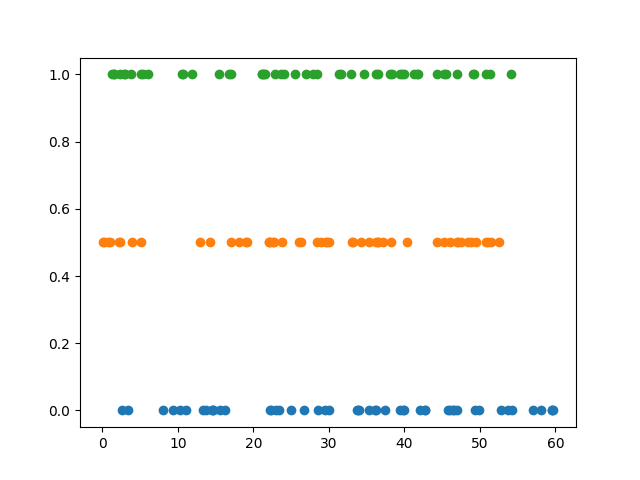
\includegraphics[width=0.75\textwidth]{poisson_sim.png}

\textcolor{red}{I think I should change this to be separate plots. Can show the intensity function for each; e.g. for inhomogenous it's the same for every realisation, but for hawkes process the intensity function is itself random.}

\subsection{Inhomogeneous Poisson Process}
An inhomogeneous Poisson process is a generalisation of the Poisson process for which the second condition is replaced by the weaker requirement that every measurable set $A\in\Sigma_T$ with finite Lebesgue measure $\mu_{\mathrm{Lebesgue}}(A)$ has a finite expectation measure, and every $A$ satisfying $\mu_\mathrm{Lebesgue}(A)=0$ also satisfies $\Lambda_\mathbb{P}(A)=0$.

By the Radon-Nikodym theorem, since $\Lambda_\mathbb{P}$ is absolutely continuous with respect to $\mu_\mathrm{Lebesgue}$, the expectation density $\lambda_\mathbb{P}$ exists. Furthermore, because the counting measure on $(t,t+\epsilon]$ is independent from the counting measure on any disjoint set, we have that $\lambda_\mathbb{P}(\omega,t)$ is adapted to the same filtration $\mathcal{F}$ as the counting process, from which it follows that the intensity process is simply $\lambda=\lambda_\mathbb{P}$ and is therefore constant with respect to $\omega$.

Since $\lambda$ is deterministic, the compensator process $\bar\Lambda$ will also be deterministic (i.e. a function of $t$ only), which allows us to simulate an inhomogenous point process by taking the random sequence $\left\{{\bar\Lambda}^{-1}(\tau(\omega)_i)\right\}_{i\in\mathbb{N}}$ for some Poisson process $\tau$, so long as the inverse function ${\bar\Lambda}^{-1}$ exists (i.e. $\bar\Lambda$ is strictly increasing).

Deterministic variation in $\lambda$ as a function of $t$ is useful for modeling deterministic seasonality in the point process, such as having more events near the start and end of each trading session, or near known events such as news releases.

\textcolor{red}{Show U-shape from empirical data}
\textcolor{red}{Show U-shape from quadratic IPP}

\subsection{Hawkes Processes}
In the case of the homogenous and inhomogenous Poisson processes, the intensity function is deterministic, i.e. constant in $\omega$. While such an assumption is appropriate for modeling the arrival of independent events, it is common in financial markets for events to ``cluster'' together in a non-deterministic fashion, with the intensity dependent on the recent historical behaviour of the point process. One explicit test for this phenomenon is to examine the autocorrelation of residuals of an inhomogenous Poisson process model, \textcolor{red}{which will be covered in some section of the applications chapter}.
\textcolor{red}{Show ACF of inter-arrival times}

The increase in intensity seen after a series of related events in quick succession is known as \textit{self-excitation}\footnote{In the case of multivariate point processes, interactions between different event types are often called \textit{cross-exciting}. The opposite behaviour, where recent occurrences temporarily decrease the intensity, is known as \textit{self-inhibition} or \textit{cross-inhibition}.}, and requires us to introduce a stochastic component to the intensity of our model that will depend on the realised history of the point process up until $t$. By analogy with time series literature, the dependence of forecasts on recent history is referred to as \textit{autoregressive}.

A popular class of autoregressive models are known as \textit{Hawkes Processes}, first introduced by 
\textcolor{red}{Original hawkes process paper https://academic.oup.com/biomet/article-abstract/58/1/83/224809?redirectedFrom=fulltext}
\textcolor{red}{Discuss history of their application to financial datasets}

Univariate Hawkes process models require that the intensity process have the functional form
$$\lambda(\omega,t) = \nu + \int_{t_\mathrm{min}}^t k(t-s)d\Lambda_\omega(s),$$
where $\nu\in\mathbb{R}_{>0}$ represents a constant arrival rate, $k$ is a kernel function encoding the impact of each event on the future intensity, and $t_\mathrm{\min}$ is the earliest time events can occur, such as the opening time of a trading session. I will assume that $k$ takes positive values for nonnegative arguments, and is zero for negative arguments. \textcolor{red}{Existence and nonexplosiveness of such processes is established... where?}
\textcolor{red}{Integral is open on the right bound of the interval of integration}

In the case of a multivariate point process $(\mathcal{T},\mathcal{E})$, we can generalise this functional form to
$$\lambda_e(\omega,t) = \nu_e + \sum_{e'} \int_{t_\mathrm{min}}^t k_{e',e}(t-s)d\Lambda_\omega^{e'}(s),$$
where $k_{e',e}$ is the kernel associated with the pair of event types $(e',e)\in E^2$. For convenience, we can arrange the $\lambda_e(\omega,t)$ and $\Lambda_\omega$ into $\vert E\vert$-dimensional vector-valued functions $\lambda(\omega,t)$ and $\Lambda_\omega$. Similarly, the base rates $\nu_e$ can be arranged into a vector $\nu$, and the functions $k_{e',e}$ into a matrix-valued function $k(t-s)$. Then finally we have
$$\lambda(\omega,t) = \nu + \int_{t_\mathrm{min}}^t k(t-s)^T d\Lambda_\omega(s).$$

Let $K(t)=\int_0^t k(u)du$.

\textcolor{red}{Since $\lambda$ can't take on negative values, the kernel function must be positive. Show also that it must have finite L1 norm}

It is possible to generate samples from a multivariate Hawkes process $(\mathcal{T},\mathcal{E})$ in the following manner. Firstly, draw samples from a multivariate Poisson process $\mathcal{T}'$ with rate $\nu$, and let $\tau_0$ be the resulting sequence of pairs $(t,e)\in T\times E$, ordered by time. For each $e$, we have the function $K_{e_i,e}$ and its inverse function $K_{e_i,e}^{-1}$. Draw samples from an independent Poisson process $\pi_i^e$ with unit rate until one of the times exceeds $K_{e_i,e}(\infty)$. Following this, let $$g_i^e=\{(K_{e_i,e}^{-1}(t)+\tau_{i,i}',e) \vert t\in\pi_i^e\},$$ where $\tau_{i,i}'$ is the time component of the pair $\tau_{i,i}$. Lastly, let $$\tau_{i+1}=\tau_i\cup \bigcup_{e\in E}g_i^e.$$ Then the sequence of pairs $\{\tau_{i,i}\}_{i\in\mathbb{N}}$ will be distributed in accordance with the desired multivariate Hawkes process. \textcolor{red}{Proof? or source? Immigration-birth interpretation \cite{MorariuPatrichiPakkanen} (aka Watson-Galton models). Introduce the term \textit{parent event}}
\textcolor{red}{Stability criterion. I think it's $\det K<1$. but how to prove. have $\bar\lambda = (I-K)^{-1}\nu$.}

For computational simplicity, it is often convenient to use a kernel of the form
$$k_{e',e}(u) = \sum_i \alpha_{e',e,i}\exp(-\beta_{e',e,i} u),$$
for some real numbers $\alpha_{e',e,i}$ and positive real numbers $\beta_{e',e,i}$.
Suppose that $k_{e',e}$ has some different functional form, but is still continuous. The Weierstrass approximation theorem guarantees that every continuous function on some closed interval can be uniformly approximated as closely desired by polynomials. Since polynomials in $\exp(-u)$ with no constant term can be written in the above form, and this is a continuous bijective function of $u$, it follows that any continuous function on a closed interval can be approximated arbitrarily well by a kernel of this form and a constant term. Since the constant term is arbitrarily well approximated by very small values of $\beta_{e',e,i}$, we can approximate any other continuous kernel function arbitrarily well by a linear combination of decreasing exponentials.
\textcolor{red}{This proof needs more detail. Use triangle inequality}

\textcolor{red}{Explain why it is better computationally}

\textcolor{red}{According to \texttt{https://ieeexplore.ieee.org/document/7416001 https://arxiv.org/pdf/1401.0903}, hawkes processes are fully determined by the first two moments of the intensity function. Proof in the paper.}

\subsection{State Dependence}
Just as the arrivals of events in the limit order book governs the evolution of its state over time, we might reasonably expect that the arrival rate of certain kinds of events is dependent on the present state of the order book, as captured by a variety of features. Vinkovskaya (2014) \cite{Vinkovskaya} proposed a regime-switching variant of the Hawkes process model for which the kernel function additionally depends on whether the market was one tick wide at the time of the parent event, finding a greater self-excitation effect for the various event types in the one-tick-wide regime.

Moriaru-Patrichi and Pakkanen (2022) \cite{MoriaruPatrichiPakkanen} find similarly that a regime-switching variant learns different parameters for the one-tick-wide regime, as well as in a model using five different states based on queue imbalance. Their work is distinguished from prior regime-switching approaches in the sense that they also model the evolution of the order book state over time as a finite state-switching process, with transition probabilities at each event time also dependent on the event type. While this coupling of a point process model with state-switching behaviour admits broader application than simple modeling of arrival times, this is not the primary focus of the work, and the simple nature of their state model leaves room for further extension.

The model of \cite{MoriaruPatrichiPakkanen} takes the form
\begin{equation}
	\lambda_e(\omega,t) = \nu_{\mathcal{X}(\omega,t),e} + \sum_{e'\in E}\int_{t_\mathrm{min}}^t k_{\mathcal{X}(\omega,s),e',e}(t-s)d\Lambda_\omega^{e'}(s), \label{eq:sdhp}
\end{equation}
where $\mathcal{X}(\omega,t)$ is a discrete-valued stochastic process representing the order book state, with jumps only at the event times of the point process.

Notably, the focus of prior work has been primarily on the case with a finite number of discrete states, possibly obtained by discretisation of a continuous quantity such as queue imbalance. Consideration of multiple state variables quickly becomes difficult, as the number of states grows exponentially in the number of independent state variables. No prior information is taken into account regarding the monotonicity of excitation with respect to continuous state variables, and no extrapolation can take place on this basis.

One deficiency of this particular model is the lack of dependence on the order book state at time $t$. Information about states is only taken into account at the times of the parent events, making the long-term effects of previous events independent of the present state. To address this, I propose a more general model of the form
$$\lambda_e(\omega,t) = \nu_{\mathcal{X}(\omega,t),e} + \sum_{e'\in E}\int_{t_\mathrm{min}}^t k_{\mathcal{X}(\omega,s),\mathcal{X}(\omega,t),e',e}(t-s)d\Lambda_\omega^{e'}(s).$$

Assuming that for each $(e',e)$ the kernel function $k_{e',e}$ is a sum of terms $k_{e',e,i}$ that are separable in $\mathcal{X}(s)$, $\mathcal{X}(t)$, and $t-s$, \textcolor{red}{explain why this assumption still lets us approximate any true situation with enough component kernels}, we obtain
\begin{equation}
	\lambda_e(\omega,t) = \nu_{\mathcal{X}(\omega,t),e} + \sum_i \sum_{e'\in E}\int_{t_\mathrm{min}}^t A_{e',e,i}(\mathcal{X}(\omega,s))B_{e',e,i}(\mathcal{X}(\omega,t))k_{e',e,i}(t-s)d\Lambda_\omega^{e'}(s). \label{eq:dual_sdhp}
\end{equation}

In the case where $A$ and $B$ are finite-valued, the state space $X$ is partitioned into a variety of discrete states. If we allow $k_{e',e,i}$ to take the same functional form as the state-dependent kernel of equation \ref{eq:sdhp}, then a model of the form \ref{eq:dual_sdhp} with one component for every state nests a model of the form \ref{eq:sdhp} by making $B_{e',e,i}$ a positive constant, and setting $A_{e',e,i}$ to $1$ if its argument is in the $i$th state or $0$ otherwise.

A further generalisation would write $A$ and $B$ as continuous functions of the order book state. A convenient choice is the form $\exp(c\cdot \chi(\mathcal{X}(\omega,t)))$, where $\chi(\mathcal{X}(\omega,t))$ is a feature vector derived from the full order book state $\mathcal{X}(t)$ and $c$ is a coefficient vector of the same size. This ensures that $A$ and $B$ are necessarily positive and captures monotonic effects of the state variables on the intensity, while still being flexibly parameterised. \textcolor{red}{If $k_{e',e,i}$ is allowed to be zero, then introducing one component per state, we can replicate the finite-state model by letting $\chi$ be a vector with one element for each state, that is one at the entry corresponding to the present state and zero elsewhere.}

\textcolor{red}{Weierstrass approximation thm again applies: with enough components, any continuous functional form for $A$ and $B$ can be uniformly well approximated on an arbitrarily large interval}

\textcolor{red}{Emphasise that this is novel}

\subsection{Raising the Intensity to a Power}
Though the Hawkes process intensity manages to capture self-exciting feedback loops in the behaviour of the point process, it may be the case that the response to a series of events is better captured by some nonlinear function. For instance, it may be the case that two identical events in close succession should contribute more or less than double to the intensity what a single event might contribute on its own, a situation that is not captured by the model as described so far.

One way to induce nonlinearity in the response function is to raise it to some positive real power $\kappa$, obtaining
$$\lambda_e(\omega,t) = \nu_e + \left(\sum_{e'\in E}\int_{t_\mathrm{min}}^t A_{e',e}(\mathcal{X}(\omega,s))B_{e',e}(\mathcal{X}(\omega,t))k_{e',e}(t-s)d\Lambda_\omega^{e'}(s)\right)^\kappa.$$

More generally, we might have a linear combination of such terms, writing
\begin{equation}
	\begin{align}
		\lambda_{e',e}^i(\omega,t) &= \int_{t_\mathrm{min}}^t A_{e',e,i}(\mathcal{X}(\omega,s))B_{e',e,i}(\mathcal{X}(\omega,t))k_{e',e,i,i}(t-s)d\Lambda_\omega^{e'}(s), \\
		\lambda_e^i(\omega,t) &= \sum_{e'\in E}\lambda_{e',e}^i(\omega,t), \\
		\lambda_e(\omega,t) &= \nu_e + \sum_i \pm_i \lambda_e^i(\omega,t)^{\kappa_i}.
	\end{align}\label{eq:general_model}
\end{equation}
\textcolor{red}{I made the background rate state-independent. Explain why I can choose very small $\kappa$ to get the same result as state-dependence.}
By taking $\kappa_j$ to be integers, and supposing that the excitation components $\lambda_e^j$ are scalar multiples of $\lambda_e^0$, we see that this nests a more restricted model where the intensity is given by some some polynomial function of $\lambda_e^0$. By the Weierstrass approximation theorem, we are therefore able to uniformly approximate an intensity formed by any continuous function of $\lambda_e^0$, so long as $\lambda_e^0$ remains within some arbitrarily large interval. In order to apply gradient-based methods in estimating $\kappa_j$, however, it is more convenient to let it be any positive real number. \textcolor{red}{but what to do if the base is negative? well, just dont let it be, force alpha to be nonnegative}

\textcolor{red}{Explain why this nests the quadratic hawkes process}
%https://arxiv.org/abs/1509.07710
\textcolor{red}{``We introduce and establish the main properties of QHawkes ("Quadratic" Hawkes) models. QHawkes models generalize the Hawkes price models introduced in E. Bacry et al. (2014), by allowing all feedback effects in the jump intensity that are linear and quadratic in past returns. A non-parametric fit on NYSE stock data shows that the off-diagonal component of the quadratic kernel indeed has a structure that standard Hawkes models fail to reproduce. Our model exhibits two main properties, that we believe are crucial in the modelling and the understanding of the volatility process: first, the model is time-reversal asymmetric, similar to financial markets whose time evolution has a preferred direction. Second, it generates a multiplicative, fat-tailed volatility process, that we characterize in detail in the case of exponentially decaying kernels, and which is linked to Pearson diffusions in the continuous limit. Several other interesting properties of QHawkes processes are discussed, in particular the fact that they can generate long memory without necessarily be at the critical point. Finally, we provide numerical simulations of our calibrated QHawkes model, which is indeed seen to reproduce, with only a small amount of quadratic non-linearity, the correct magnitude of fat-tails and time reversal asymmetry seen in empirical time series.''}

\textcolor{red}{computational details covered in estimation section}


\chapter{Estimation}%\label{something}
Selecting a model from some parametric family of point process models based on empirical order book data serves two primary purposes. Firstly, estimating the parameters of a sufficiently parsimonious and interpretable model serves to provide direct insight into the relationship between various order book events and states, such as by identifying the sign of various parameters, comparing the magnitude of parameters to one another, and performing hypothesis tests to see if a parameter is significantly different from some default value. From this we may tentatively draw qualitative conclusions about the true behaviour of the data generating process governing market behaviour. Secondly, by estimating both a point process model and a model for state transitions at each event time, we can identify a model that will allow us to simulate synthetic order book data in a manner reasonably consistent with actual market behaviour. Repeated samples from a simulation of true market behaviour may be used to predict the evolution of the order book from some initial market state, or to answer counterfactual questions such as the effect of placing a trade with some quantity at some point in time \textcolor{red}{in the same way that the Santa Fe model implies a price impact model in the paper that proposed it}.

In this thesis I will focus on maximum likelihood estimation from parametric families, using a quasi-Newton variant of the EM algorithm that updates parameters iteratively based on the gradient of the loglikelihood and the diagonal of its hessian. \textcolor{red}{is this accurate}

\section{Empirical Likelihood}
I will work with a dataset of the form $\mathcal{D} = \left(\mathcal{T}_\mathrm{obs},\mathcal{X}_\mathrm{obs}\right)$, consisting of a sequence of event times and event marks observed in the time interval $$[t_\mathrm{min},t_\mathrm{max}].$$
We can define a counting measure $\Lambda_\mathcal{D}$ on the space of events times $(T,\Sigma_T)$ by
$$\Lambda_{\mathcal{D}} : \Sigma_T \to \mathbb{R}_{\geq 0}$$
$$\Lambda_{\mathcal{D}}(A) \coloneq \left\vert A\cap\mathcal{T}_\mathrm{obs}\right\vert.$$

Similarly, we can define a càdlàg counting function
$$N_\mathcal{D} : T \to \mathbb{N}$$
$$N_\mathcal{D}(t) \coloneq \left\vert \mathcal{T}_\mathrm{obs}\cap [t_\mathrm{min},t]\right\vert = \int_{[t_\mathrm{min},t]} d\Lambda_\mathcal{D}.$$

In the multivariate case we will further have $\Lambda_\mathcal{D}^e$ and $N_\mathcal{D}^e$ for each event type $e$.

Given a subset of the data $\mathcal{D}_t$ containing only the event times and marks up until some time $t$, it is reasonable to ask whether we can predict the remainder of the dataset using some model of the point process that generated the data.

\subsection{Empirical Intensity and Loglikelihood}
If we consider a point process $\mathcal{T}$ defined with respect to $\mathbb{P}$ and having natural filtration $\mathcal{F}$, we can construct an \textit{empirical intensity function}
$$\lambda_\mathcal{D}(t) \coloneq \lambda_{\mathbb{P}\vert\mathcal{F}_t,\mathcal{D}_t}(t)$$
as the intensity conditional on the $\sigma$-algebra $\mathcal{F}_t$ and the contents of $\mathcal{D}_t$. For the point processes considered in this thesis, we have formulae representing $\lambda(\omega,t)$ as an expression involving $t$, $\mathcal{X}$, and the counting measure $\Lambda_\omega$ restricted to $[t_\mathrm{min},t)$. In this setting, it suffices to replace $\Lambda_\omega$ with $\Lambda_\mathcal{D}$ in order to compute the empirical intensity function, from which we can proceed to compute the loglikelihood of some model with reference to the event times (conditional on the marks), given in equation 7.1.2 of \cite{DaleyVereJones} as
\begin{equation}
	\begin{align}
		\ell_\mathcal{D} = \int_{t_\mathrm{min}}^{t_\mathrm{min}} \log\left(\lambda_\mathcal{D}(t)\right)d\Lambda_\mathcal{D}(t) - \int_{t_\mathrm{min}}^{t_\mathrm{min}} \lambda_\mathcal{D}(t)dt.
	\end{align}
\end{equation}

In the case of a multivariate point process, the empirical intensity function will be a vector with elements $\lambda_\mathcal{D}^e(t)$, and the loglikelihood will be given by
\begin{equation}
	\begin{align}
		\ell_\mathcal{D} = \sum_e \left(\int_{t_\mathrm{min}}^{t_\mathrm{min}} \log\left(\lambda_\mathcal{D}^e(t)\right)d\Lambda_\mathcal{D}(t) - \int_{t_\mathrm{min}}^{t_\mathrm{min}} \lambda_\mathcal{D}^e(t)dt\right).
	\end{align}
\end{equation}


\textcolor{red}{maybe point out that even defining what loglikelihood means for a point process is nontrivial and refer to the relevant section of \cite{DaleyVereJones} for more detail}
If we have access to multiple empirical datasets $\mathcal{D}_1,\mathcal{D}_2,\ldots,\mathcal{D}_n$ representing independent realisations of some underlying data generating process, the loglikelihood of the combined dataset $\mathcal{D}_\mathrm{all}$ is simply $\sum_{i=1}^n \ell_{\mathcal{D}_i}$.

\section{Maximum Likelihood Estimation}
Given a parametric family of marked multivariate point processes,
$$\{(\mathcal{T}_\theta,\mathcal{X}) : \theta\in\Theta\},$$
we wish to select one model from the family that best describes the empirical data.

Because the likelihood function tells us the probability density of the observed data under the corresponding model, a higher likelihood function corresponds to a better fit of model to data. Assuming that the likelihood has a unique global maxima
$$\hat\theta_\mathrm{MLE}(\mathcal{D}_\mathrm{all}) \coloneq \argmax_\theta L(\theta;\mathcal{D}),$$
this quantity is known as the \textit{maximum likelihood estimate} for $\theta$, and is a popular method of selecting a single ``best'' model from a parametric family.

For any point process $\mathcal{T}_\theta$ in the family, as well as some model for the marks $\mathcal{X}$, we can construct a synthetic dataset $\mathcal{D}'$. Then $\hat\theta_\mathrm{MLE}(\mathcal{D}_\mathrm{all})$ is a random variable.

As the number of independent realisations $n$ grows, we have the classical result that
$$\sqrt{n}\left(\hat\theta_\mathrm{MLE}(\mathcal{D}_\mathrm{all})-\theta\right) \to_\mathbb{P} \mathcal{N}(0,\mathcal{I}(\theta)^{-1}),$$
where $\mathcal{I}(\theta)$ is the Fisher information matrix. Furthermore, it is demonstrated in \cite{Ogata1977}, that even for a single realisation of a point process model, the MLE is consistent and asymptotically normal as the size of the observation interval $[t_\mathrm{min},t_\mathrm{max}]$ grows, in the sense that
$$\sqrt{t_\mathrm{max}-t_\mathrm{min}}\left(\hat\theta_\mathrm{MLE}(\mathcal{D}_\mathrm{all})-\theta\right) \to_\mathbb{P} \mathcal{N}(0,\mathcal{I}(\theta)^{-1}),$$
\textcolor{red}{maybe double check this}
under a permissive set of assumptions satisfied by all the models considered in this thesis.

Because finding global maxima is in general a hard problem, it is common to first weaken our search to finding stationary points of $\ell_{\mathcal{D}_\mathrm{all}}(\theta)$ using the gradient vector $\nabla_\theta \ell_{\mathcal{D}_\mathrm{all}}(\theta)$. We can then check whether the hessian matrix $H_\theta\ell_{\mathcal{D}_\mathrm{all}}(\theta)$ satisfies the requirement of negative definiteness, eliminating local minima and saddle points. Finally, we can select the best local maxima among those found in the hope that either it is the global maxima, or that it has a similar enough likelihood to the true $\hat\theta_\mathrm{MLE}$ to be a good model choice.

Note that the gradient and hesssian of $\ell_{\mathcal{D}_\mathrm{all}}$ will be the sum of the gradients (respectively, hessians) for each $\ell_{\mathcal{D}_i}$, $i=1,2,\ldots n$. So it suffices to consider a single realisation $\mathcal{D}$, for which each point process $\mathcal{T}_\theta$ will have an associated empirical intensity $\lambda_\mathcal{D}^\theta(t)$ with entries $\lambda_\mathcal{D}^{\theta,e}(t)$ at each time $t$. Then we will have
\begin{equation}
	\begin{align}
		\nabla_\theta \ell_\mathcal{D}(\theta) &= \sum_e\left(\int_{t_\mathrm{min}}^{t_\mathrm{max}}\nabla_\theta \log(\lambda_\mathcal{D}^{\theta,e}(t))d\Lambda_\mathcal{D}(t)-\int_{t_\mathrm{min}}^{t_\mathrm{max}}\nabla_\theta \lambda_\mathcal{D}^{\theta,e}(t) dt\right)\\
		&= \sum_e\left(\int_{t_\mathrm{min}}^{t_\mathrm{max}} \frac{\nabla_\theta \lambda_\mathcal{D}^{\theta,e}(t)}{\lambda_\mathcal{D}^{\theta,e}(t)} d\Lambda_\mathcal{D}(t)-\int_{t_\mathrm{min}}^{t_\mathrm{max}}\nabla_\theta \lambda_\mathcal{D}^{\theta,e}(t) dt\right),\\
		H_\theta \ell_\mathcal{D}(\theta) &= \sum_e\left(\int_{t_\mathrm{min}}^{t_\mathrm{max}} H_\theta \log(\lambda_\mathcal{D}^{\theta,e}(t))d\Lambda_\mathcal{D}(t) - \int_{t_\mathrm{min}}^{t_\mathrm{max}} H_\theta \lambda_\mathcal{D}^{\theta,e}(t) dt\right)\\ 
		&= \sum_e\left(\int_{t_\mathrm{min}}^{t_\mathrm{max}} \left( \frac{H_\theta \lambda_\mathcal{D}^{\theta,e}(t)}{\lambda_\mathcal{D}^{\theta,e}(t)} - \left\|\frac{\nabla_\theta\lambda_\mathcal{D}^{\theta,e}(t)}{\lambda_\mathcal{D}^{\theta,e}(t)}\right\|^2 \right) d\Lambda_\mathcal{D}(t) - \int_{t_\mathrm{min}}^{t_\mathrm{max}} H_\theta \lambda_\mathcal{D}^{\theta,e}(t) dt\right).\\ 
	\end{align}
\end{equation}

\textcolor{red}{explain that I will use a quasi newton method to maximise loglikelihood}

\subsection{Poisson Processes}
Suppose we have a family of multivariate Poisson process models parameterised by their constant intensity vector $\nu$ with components $\nu_e$. The log-likelihood of each model is then given by
\begin{equation}
	\begin{align}
		\ell_\mathcal{D}(\nu) &= \sum_e \left(\int_{t_\mathrm{min}}^{t_\mathrm{max}}\log(\nu_e)d\Lambda_\mathcal{D}-\int_{t_\mathrm{min}}^{t_\mathrm{max}}\nu_e dt\right)\\
		&= \sum_e \left( \log(\nu)\int_{t_\mathrm{min}}^{t_\mathrm{max}}d\Lambda_\mathcal{D} - \nu\int_{t_\mathrm{min}}^{t_\mathrm{max}}dt \right)\\
		&= \sum_e \left(\log(\nu)N_\mathcal{D}\left(t_\mathrm{max}\right) - \nu\left(t_\mathrm{max}-t_\mathrm{min}\right)\right).
	\end{align}
\end{equation}

This implies that
\begin{equation}
	\begin{align}
		\frac{\partial}{\partial\nu_e}\ell_\mathcal{D}(\nu) = \frac{1}{\nu_e}N_\mathcal{D}\left(t_\mathrm{max}\right)-\left(t_\mathrm{max}-t_\mathrm{min}\right) \\
		\frac{\partial}{\partial\nu_e\partial\nu_{e'}}\ell_\mathcal{D}(\nu) = -\delta_{e,e'}\frac{N_\mathcal{D}\left(t_\mathrm{max}\right)}{\nu_e^2} \leq 0, \\
	\end{align}
\end{equation}
where $\delta_{e,e'}$ is $1$ if and only if $e=e'$ and $0$ otherwise.

Since the hessian is a diagonal matrix with negative diagonal entries, it is negative definite, and so a unique local maxima exists and is a global maxima. Using the fact that $\nabla_\nu \ell_\mathcal{D}(\nu)=0$, we obtain
\begin{equation}
	\hat\nu_\mathrm{MLE} = \frac{N_\mathcal{D}(t_\mathrm{max})}{t_\mathrm{max}-t_\mathrm{min}}.
\end{equation}

Intuitively, the estimate for the arrival rate $\nu$ is the average number of events per unit time in the observed data. Note also that for the maximum likelihood model, the sample average of the residuals $r$ will be exactly equal to one, since we have
$$\sum_{i=1}^{N_\mathcal{D}(t_\mathrm{max})} r_i = \bar\Lambda(t_\mathrm{max})=\hat\nu_\mathrm{MLE}(t_\mathrm{max}-t_\mathrm{min}) =N_\mathcal{D}(t_\mathrm{max}).$$

\section{Maximum Likelihood Estimation for Composite Processes}
Suppose that for each point process $\mathcal{T}_\theta$ in a parametric family we have
$$\lambda^\theta(\omega,t)=\sum_i \lambda^{i,\theta^i}(\omega,t),$$
where the parameter vector $\theta$ may be written as a concatenation of the parameter vectors $\theta^i$ governing the terms $\lambda^{i,\theta^i}(\omega,t)$. Then we will have empirical component probabilities $P_{\mathcal{D},i}$ with elements
$$P_{\mathcal{D},i}^e(t) = \frac{\lambda_\mathcal{D}^{i,\theta^i,e}(t)}{\lambda_\mathcal{D}^e(t)}.$$

It follows that
\begin{equation}
	\begin{align}
		\nabla_{\theta^i} \ell_\mathcal{D}(\theta) &= \sum_e\left(\int_{t_\mathrm{min}}^{t_\mathrm{max}} \frac{\nabla_{\theta^i} \lambda_\mathcal{D}^{i,\theta^i,e}(t)}{\lambda_\mathcal{D}^{\theta,e}(t)} d\Lambda_\mathcal{D}(t)-\int_{t_\mathrm{min}}^{t_\mathrm{max}}\nabla_{\theta^i} \lambda_\mathcal{D}^{\theta,e}(t) dt\right) \\
		&= \sum_e\left(\int_{t_\mathrm{min}}^{t_\mathrm{max}} \frac{\nabla_{\theta^i} \lambda_\mathcal{D}^{i,\theta^i,e}(t)}{\lambda_\mathcal{D}^{i,\theta^i,e}(t)}\cdot\frac{\lambda_\mathcal{D}^{i,\theta^i,e}(t)}{\lambda_\mathcal{D}^{\theta,e}(t)} d\Lambda_\mathcal{D}(t)-\int_{t_\mathrm{min}}^{t_\mathrm{max}}\nabla_{\theta^i} \lambda_\mathcal{D}^{\theta,e}(t) dt\right) \\
		&= \sum_e\left(\int_{t_\mathrm{min}}^{t_\mathrm{max}} \nabla_{\theta^i} \log\left(\left\vert \lambda_\mathcal{D}^{i,\theta^i,e}(t) \right\vert\right)\cdot P_{\mathcal{D},i}^e(t) d\Lambda_\mathcal{D}(t)-\int_{t_\mathrm{min}}^{t_\mathrm{max}}\nabla_{\theta^i} \lambda_\mathcal{D}^{\theta,e}(t) dt\right) \\
		H_{\theta^i} \ell_\mathcal{D}(\theta) &= \sum_e \int_{t_\mathrm{min}}^{t_\mathrm{max}} \left( \frac{H_{\theta^i} \lambda_\mathcal{D}^{i,\theta^i,e}(t)}{\lambda_\mathcal{D}^{i,\theta^i,e}(t)} - \frac{ \left(\nabla_{\theta^i}\lambda_\mathcal{D}^{i,\theta^i,e}(t)\right) \left(\nabla_{\theta^i}\lambda_\mathcal{D}^{i,\theta^i,e}(t)\right)^T  }{\lambda_\mathcal{D}^{i,\theta^i,e}(t)^2} \cdot P_{\mathcal{D},i}^e(t)\right)\cdot P_{\mathcal{D},i}^e(t) d\Lambda_\mathcal{D}(t) \\ &- \sum_e\int_{t_\mathrm{min}}^{t_\mathrm{max}} H_\theta \lambda_\mathcal{D}^{i,\theta^i,e}(t) dt,\\ 
	\end{align}\label{eq:derivatives}
\end{equation}
where $\lambda^{i,\theta^i,e}(\omega,t)$ are the elements of the vector $\lambda^{i,\theta^i}(\omega,t)$. The full gradient $\nabla_\theta \ell_\mathcal{D}(\theta)$ is then the concatenation of the individual gradients $\nabla_{\theta^i} \ell_\mathcal{D}(\theta)$, and similarly the hessian $H_\theta \ell_\mathcal{D}(\theta)$ will be a block-diagonal matrix with $H_{\theta^i}\ell_\mathcal{D}(\theta)$ placed in the block whose rows and columns correspond to $\theta^i$, and zeros in the remaining entries.

\subsection{Expectation Maximisation}
\textcolor{red}{Not sure if I will include this!}
If $\left(\lambda_i^{\theta_i}\right)_\mathcal{D}$ are positive, we have
$$\log\left(\sum_i \left(\lambda_i^{\theta_i}\right)_{\mathcal{D}}(t)\right) = \sum_i \log\left(\left(\lambda_i^{\theta_i}\right)_\mathcal{D}(t)\right)B_{i,t}^{\theta_1,\theta_2,\ldots} - \sum_i \log\left( B_{i,t}^{\theta_1,\theta_2,\ldots}\right)B_{i,t}^{\theta_2,\theta_2,\ldots},$$
By Gibb's inequality, it follows that
$$- \sum_i \log\left( B_{i,t}^{\theta_1,\theta_2,\ldots}\right)B_{i,t}^{\theta_1,\theta_2,\ldots} \leq - \sum_i \log\left( B_{i,t}^{\theta_1',\theta_2',\ldots}\right)B_{i,t}^{\theta_1,\theta_2,\ldots} $$

\textcolor{red}{EM algorithm and proof of convergence.}

\textcolor{red}{Can cite original dempster paper? As well as the one that corrects the errors in that paper}

\textcolor{red}{- Equations

- Visualisation of branching matrix. How does it evolve throughout the fitting procedure?

- Quasi EM approximation

- Closed form constant time M step for multivariate state dependent hawkes processes

- Method of scoring (Newton's method)

- Negative probabilities. Conditions for kernel nonnegativity? (Probably not tractable) }

\section{General Point Process Model}
Recall that the model with component intensities raised to powers $\kappa_i$ was so far the most general model, nesting all others described. I will therefore focus my attention on this model with the intention that results for the simpler models will follow from this analysis. Recall the intensity as described in \eqref{eq:general_model},
\begin{equation*}
	\begin{align}
		\lambda_e(\omega,t) &= \nu_e + \sum_i \pm_i \lambda_e^i(\omega,t)^{\kappa_i}, \\
		\lambda_e^i(\omega,t) &= \sum_{e'\in E}, \\
		\lambda_{e',e}^i(\omega,t) &= \int_{t_\mathrm{min}}^t A_{e',e,i}(\mathcal{X}(\omega,s))B_{e',e,i}(\mathcal{X}(\omega,t))k_{e',e,i,i}(t-s)d\Lambda_\omega^{e'}(s).
	\end{align}
\end{equation*}

To be more concrete, I will consider an intensity of the form
\begin{equation}
	\begin{align}
		\lambda_e(\omega,t) &= \nu_e + \sum_i \pm_i \lambda_e^i(\omega,t)^{\kappa_i}, \\
		\lambda_e^j(\omega,t) &= \sum_{e'\in E} \lambda_{e',e}^j(\omega,t), \\
		\lambda_{e',e}^j(\omega,t) &= \int_{t_\mathrm{min}}^t \alpha_{e',e,i} A_{e',e,i}(\omega,s) B_{e',e,i}(\omega,t)\exp(-\beta_i(t-s))d\Lambda_\omega^{e'}(s), \\
		A_{e',e,i}(\omega,s) &= \exp(a_{e',e,i}\cdot\chi(\mathcal{X}(\omega,s))), \\
		B_{e',e,i}(\omega,t) &= \exp(b_{e',e,i}\cdot\chi(\mathcal{X}(\omega,t))).
	\end{align}
\end{equation}

This is parameterised by $\nu,\alpha,\beta,a,b,\kappa$.

On some dataset $\mathcal{D}$, the empirical intensity will then have the form
\begin{equation}
	\begin{align}
		\lambda_\mathcal{D}^e(t) &= \nu_e + \sum_i \pm_i \lambda_\mathcal{D}^{i,e}(t)^{\kappa_i}, \\
		\lambda_\mathcal{D}^{e,i}(t) &= \sum_{e'\in E} \lambda_\mathcal{D}^{e',e,i}(t) \\
		\lambda_\mathcal{D}^{e',e,i}(t) &= \int_{t_\mathrm{min}}^t \alpha_{e',e,i} A_\mathcal{D}^{e',e,i}(s) B_\mathcal{D}^{e',e,i}(t)\exp(-\beta_i(t-s))d\Lambda_\mathcal{D}^{e'}(s), \\
		A_\mathcal{D}^{e',e,i}(s) &= \exp(a_{e',e,i}\cdot\chi(\mathcal{X}_\mathcal{D}(s))), \\
		B_\mathcal{D}^{e',e,i}(t) &= \exp(b_{e',e,i}\cdot\chi(\mathcal{X}_\mathcal{D}(t))),
	\end{align}
\end{equation}
where $\mathcal{X}_\mathcal{D}(t)$ represents the most recent recorded state of the order book at time $t$.

\subsection{Differentiating with respect to the Parameters}
Treating $\nu_e$ as the $0$th component intensities and $\pm_i \lambda_\mathcal{D}^{i,e}^{\kappa_i}$ as the $i$th, we can write down component probabilities
\begin{equation}
	\begin{align}
		P_{\mathcal{D},0}^e(t) &= \frac{\nu_e}{\lambda_\mathcal{D}^e(t)}, \\
		P_{\mathcal{D},i}^e(t) &= \frac{\pm_i \lambda_\mathcal{D}^{e,i}(t)^{\kappa_i}}{\lambda_\mathcal{D}^e(t)}.
	\end{align}
\end{equation}

From here, we can compute derivatives of $\ell_\mathcal{D}$ with respect to each parameter, as in equation \eqref{eq:derivatives}, in order to determine \textcolor{red}{the newton step?}.

\begin{equation}
	\begin{align}
		\frac{\partial}{\partial \nu_e}\ell_\mathcal{D} &= \frac{1}{\nu_e} \int_{t_\mathrm{min}}^{t_\mathrm{max}} P_{\mathcal{D},0}^e(t)d\Lambda_\mathcal{D}^e(t) - \int_{t_\mathrm{min}}^{t_\mathrm{max}} dt \\
		&= \frac{1}{\nu_e} \int_{t_\mathrm{min}}^{t_\mathrm{max}} P_{\mathcal{D},0}^e(t)d\Lambda_\mathcal{D}^e(t) - (t_\mathrm{max}-t_\mathrm{min}), \\
		\frac{\partial^2}{(\partial \nu_e)^2}\ell_\mathcal{D} &= -\frac{1}{\nu_e^2} \int_{t_\mathrm{min}}^{t_\mathrm{max}} P_{\mathcal{D},0}^e(t)d\Lambda_\mathcal{D}^e(t), \\
	\end{align}
\end{equation}

By writing $\lambda_\mathcal{D}^{e',e,i}(t)$ as
$$\exp(-\beta_i t)\alpha_{e',e,i} B_\mathcal{D}^{e',e,i}(t)\int_{t_\mathrm{min}}^t A_\mathcal{D}^{e',e,i}(s) \exp(\beta_i s)d\Lambda_\mathcal{D}^{e'}(s),$$
it becomes evident that 
\begin{equation*}
	\begin{align}
		\lambda_\mathcal{D}^{e',e,i}(t+\epsilon) &= \exp(-\beta\epsilon) \lambda_\mathcal{D}^{e',e,i}(t), \\
		\lambda_\mathcal{D}^{e,i}(t+\epsilon) &= \exp(-\beta\epsilon) \lambda_\mathcal{D}^{e,i}(t), \\
		\pm_i\lambda_\mathcal{D}^{e,i}(t+\epsilon)^{\kappa_i} &= \pm_i \exp(-\beta\kappa_i\epsilon) \lambda_\mathcal{D}^{e,i}(t)^{\kappa_i}, \\
	\end{align}
\end{equation*}
for any $\epsilon>0$ so long as $\sum_{e'}\Lambda_\mathcal{D}^{e'}((t,t+\epsilon))=0$.
On the other hand, at some event time $t$ with event type $e$, the right-limit of $\lambda_\mathcal{D}^{e',e,i}$ will be equal to
\begin{equation}
	\begin{align}
		\lambda_\mathcal{D}^{e',e,i}(t^+) &= \frac{B_\mathcal{D}^{e',e,i}(t)}{B_\mathcal{D}^{e',e,i}(t^-)}\lambda_\mathcal{D}^{e',e,i}(t) + \alpha_{e',e,i} A_\mathcal{D}^{e',e,i}(t)B_\mathcal{D}^{e',e,i}(t),
	\end{align}
\end{equation}
where $B_\mathcal{D}^{e',e,i}(t^-)$ is the left-limit of $B_\mathcal{D}^{e',e,i}$.

Partition the observation interval $(t_\mathrm{min},t_\mathrm{max})$ into $\vert\mathcal{D}\vert+1$ different intervals $T_j$ with endpoints in $\mathcal{D}\cup\{t_\mathrm{min},t_\mathrm{max}\}$. Furthermore, define
\begin{equation}
	\begin{align}
		\Gamma_0^\gamma(T_j) &= \int_{\inf T_j}^{\sup T_j}\exp(-\gamma (t-\inf T_j))dt \\
		&= \frac{1}{\gamma} (1 - \exp(-\gamma \mu_\mathrm{Lebesgue}(T_j))), \\
		\Gamma_1^\gamma(T_j) &= \int_{\inf T_j}^{\sup T_j}(t-\inf T_j)\exp(-\gamma (t-\inf T_j))dt \\
		&= \frac{1}{\gamma^2} (1 - \exp(-\gamma \mu_\mathrm{Lebesgue}(T_j))(\gamma \mu_\mathrm{Lebesgue}(T_j) + 1)), \\
		\Gamma_2^\gamma(T_j) &= \int_{\inf T_j}^{\sup T_j}(t-\inf T_j)^2\exp(-\gamma (t-\inf T_j))dt \\
		&= \frac{1}{\gamma^3} (2 - \exp(-\gamma \mu_\mathrm{Lebesgue}(T_j))(\gamma^2\mu_\mathrm{Lebesgue}(T_j)^2+2\gamma \mu_\mathrm{Lebesgue}(T_j)+2)), \\
	\end{align}
\end{equation}
with $\mu_\mathrm{Lebesgue}(T_j) = \sup T_j - \inf T_j$.

Then differentiating with respect to $\alpha_{e',e,i}$ yields
\begin{equation*}
	\begin{align}
		\frac{\partial}{\partial\alpha_{e',e,i}} \lambda_\mathcal{D}^{e,i}(t)^{\kappa_i} &= \frac{\kappa_i}{\alpha_{e',e,i}} \lambda_\mathcal{D}^{e',e,i}(t) \lambda_\mathcal{D}^{e,i}(t)^{\kappa_i-1} \\
		\frac{\partial}{\partial\alpha_{e',e,i}}\ell_\mathcal{D} &= \int_{t_\mathrm{min}}^{t_\mathrm{max}} \frac{\kappa_i \lambda_\mathcal{D}^{e',e,i}(t)}{\alpha_{e',e,i}\lambda_\mathcal{D}^{e,i}(t)} \cdot P_{\mathcal{D},i}^e(t) d\Lambda_\mathcal{D}^e(t) - \pm_i \frac{\kappa_i}{\alpha_{e',e,i}} \int_{t_\mathrm{min}}^{t_\mathrm{max}} \lambda_\mathcal{D}^{e',e,i}(t)\lambda_\mathcal{D}^{e,i}(t)^{\kappa_i-1}dt \\
		&= \int_{t_\mathrm{min}}^{t_\mathrm{max}} \frac{\kappa_i \lambda_\mathcal{D}^{e',e,i}(t)}{\alpha_{e',e,i}\lambda_\mathcal{D}^{e,i}(t)} \cdot P_{\mathcal{D},i}^e(t) d\Lambda_\mathcal{D}^e(t) \\
		&- \pm_i \frac{\kappa_i}{\alpha_{e',e,i}} \sum_j \lambda_\mathcal{D}^{e',e,i}((\inf T_j)^+)\lambda_\mathcal{D}^{e,i}((\inf T_j)^+)^{\kappa_i-1} \Gamma_0^{\beta_i\kappa_i}(T_j), \\
		\frac{\partial^2}{(\partial\alpha_{e',e,i})^2} \lambda_\mathcal{D}^{e,i}(t)^{\kappa_i} &= \frac{\kappa_i(\kappa_i-1)}{\alpha_{e',e,i}^2} \lambda_\mathcal{D}^{e',e,i}(t)^2 \lambda_\mathcal{D}^{e,i}(t)^{\kappa_i-2}  \\
		\frac{\partial^2}{(\partial\alpha_{e',e,i})^2}\ell_\mathcal{D} &= \int_{t_\mathrm{min}}^{t_\mathrm{max}} \left( \frac{\kappa_i(\kappa_i-1)\lambda_\mathcal{D}^{e',e,i}(t)^2}{\alpha_{e',e,i}^2\lambda_\mathcal{D}^{e,i}(t)^2} - \left(\frac{\kappa_i \lambda_\mathcal{D}^{e',e,i}(t)}{\alpha_{e',e,i}\lambda_\mathcal{D}^{e,i}(t)}\right)^2 \cdot P_{\mathcal{D},i}^e(t) \right) \cdot P_{\mathcal{D},i}^e(t) d\Lambda_\mathcal{D}^e(t) \\
		&- \pm_i \int_{t_\mathrm{min}}^{t_\mathrm{max}} \frac{\kappa_i(\kappa_i-1)}{\alpha_{e',e,i}^2} \lambda_\mathcal{D}^{e',e,i}(t)^2 \lambda_\mathcal{D}^{e,i}(t)^{\kappa_i-2} dt \\
		&= \int_{t_\mathrm{min}}^{t_\mathrm{max}} \left( \frac{\kappa_i(\kappa_i-1)\lambda_\mathcal{D}^{e',e,i}(t)^2}{\alpha_{e',e,i}^2\lambda_\mathcal{D}^{e,i}(t)^2} - \left(\frac{\kappa_i \lambda_\mathcal{D}^{e',e,i}(t)}{\alpha_{e',e,i}\lambda_\mathcal{D}^{e,i}(t)}\right)^2 \cdot P_{\mathcal{D},i}^e(t) \right) \cdot P_{\mathcal{D},i}^e(t) d\Lambda_\mathcal{D}^e(t) \\
		&- \pm_i \sum_j \frac{\kappa_i(\kappa_i-1)}{\alpha_{e',e,i}^2} \lambda_\mathcal{D}^{e',e,i}((\inf T_j)^+)^2 \lambda_\mathcal{D}^{e,i}(\inf T_j)^+)^{\kappa_i-2} \Gamma_0^{\beta_i\kappa_i}(T_j). \\
	\end{align}
\end{equation*}

Next, we will have
\begin{equation*}
	\begin{align}
		\frac{\partial}{\partial\beta_i}\lambda_\mathcal{D}^{e',e,i}(t) &= -\int_{t_\mathrm{min}}^t (t-s) \alpha_{e',e,i}A_\mathcal{D}^{e',e,i}(s)B_\mathcal{D}^{e',e,i}(t)\exp(-\beta_i(t-s)) d\Lambda_\mathcal{D}^{e'}(s), \\
		\frac{\partial^2}{(\partial\beta_i)^2}\lambda_\mathcal{D}^{e',e,i}(t) &= \int_{t_\mathrm{min}}^t (t-s)^2 \alpha_{e',e,i}A_\mathcal{D}^{e',e,i}(t)B_\mathcal{D}^{e',e,i}(t)\exp(-\beta_i(t-s)) d\Lambda_\mathcal{D}^{e'}(s), \\
	\end{align}
\end{equation*}
and in the case where $\sum_{e'}\Lambda_\mathcal{D}^{e'}((t,t+\epsilon))=0$ we can express these recursively as
\begin{equation*}
	\begin{align}
		\frac{\partial}{\partial\beta_i}\lambda_\mathcal{D}^{e',e,i}(t+\epsilon) &= \exp(-\beta_i \epsilon)\left( -\epsilon\lambda_\mathcal{D}^{e',e,i}(t) + \frac{\partial}{\partial\beta_i}\lambda_\mathcal{D}^{e',e,i}(t) \right), \\
		\frac{\partial^2}{(\partial\beta_i)^2}\lambda_\mathcal{D}^{e',e,i}(t+\epsilon) &= \exp(-\beta_i \epsilon)\left( \epsilon^2\lambda_\mathcal{D}^{e',e,i}(t) - 2\epsilon\frac{\partial}{\partial\beta_i}\lambda_\mathcal{D}^{e',e,i}(t) + \frac{\partial^2}{(\partial\beta_i)^2}\lambda_\mathcal{D}^{e',e,i}(t) \right).
	\end{align}
\end{equation*}

Using these results, we can then express the derivatives of $\lambda_\mathcal{D}^{e,i}$ and $\ell_\mathcal{D}$ with respect to $\beta_i$ as
\begin{equation*}
	\begin{align}
		\frac{\partial}{\partial\beta_i} \lambda_\mathcal{D}^{e,i}(t)^{\kappa_i} &= \kappa_i \lambda_\mathcal{D}^{e,i}(t)^{\kappa_i-1} \sum_{e'} \frac{\partial}{\partial\beta_i}\lambda_\mathcal{D}^{e',e,i}(t), \\
		\frac{\partial}{\partial\beta_i}\ell_\mathcal{D} &= \int_{t_\mathrm{min}}^{t_\mathrm{max}} \frac{\kappa_i \sum_{e'} \frac{\partial}{\partial\beta_i}\lambda_\mathcal{D}^{e',e,i}(t)}{\lambda_\mathcal{D}^{e,i}(t)} P_{\mathcal{D},i}^e(t)d\Lambda_\mathcal{D}^e(t) \\
		&- \pm_i \kappa_i \int_{t_\mathrm{min}}^{t_\mathrm{max}} \lambda_\mathcal{D}^{e,i}(t)^{\kappa_i-1}\sum_{e'}\frac{\partial}{\partial\beta_i}\lambda_\mathcal{D}^{e',e,i}(t) dt \\
		&= \int_{t_\mathrm{min}}^{t_\mathrm{max}} \frac{\kappa_i \sum_{e'} \frac{\partial}{\partial\beta_i}\lambda_\mathcal{D}^{e',e,i}(t)}{\lambda_\mathcal{D}^{e,i}(t)} P_{\mathcal{D},i}^e(t)d\Lambda_\mathcal{D}^e(t) \\
		&+ \pm_i \kappa_i \sum_j \lambda_\mathcal{D}^{e,i}((\inf T_j)^+)^{\kappa_i-1}\sum_{e'} \lambda_\mathcal{D}^{e',e,i}((\inf T_j)^+)\Gamma_1^{\beta_i\kappa_i}(T_j) \\
		&- \pm_i \kappa_i \sum_j \lambda_\mathcal{D}^{e,i}((\inf T_j)^+)^{\kappa_i-1}\sum_{e'} \frac{\partial}{\partial\beta_i}\lambda_\mathcal{D}^{e',e,i}(\inf T_j)^+) \Gamma_0^{\beta_i\kappa_i}(T_j), \\
		\frac{\partial^2}{(\partial\beta_i)^2} \lambda_\mathcal{D}^{e,i}(t)^{\kappa_i} &= \kappa_i(\kappa_i-1) \lambda_\mathcal{D}^{e,i}(t)^{\kappa_i-2} \left(\sum_{e'} \frac{\partial}{\partial\beta_i}\lambda_\mathcal{D}^{e',e,i}(t)\right)^2 + \kappa_i \lambda_\mathcal{D}^{e,i}(t)^{\kappa_i-1} \sum_{e'} \frac{\partial^2}{(\partial\beta_i)^2}\lambda_\mathcal{D}^{e',e,i}(t), \\\
		\frac{\partial^2}{(\partial\beta_i)^2}\ell_\mathcal{D} &= \int_{t_\mathrm{min}}^{t_\mathrm{max}} \left( \kappa_i(\kappa_i-1)\left(\frac{\sum_{e'}\frac{\partial}{\partial\beta_i}\lambda_\mathcal{D}^{e',e,i}(t)}{\lambda_\mathcal{D}^{e,i}(t)}\right)^2 + \kappa_i \frac{\sum_{e'}\frac{\partial^2}{(\partial\beta_i)^2}}{\lambda_\mathcal{D}^{e,i}(t)} \right) P_{\mathcal{D},i}^e(t) d\Lambda_\mathcal{D}^e(t) \\
		&- \int_{t_\mathrm{min}}^{t_\mathrm{max}} \kappa_i^2\left(\frac{\sum_{e'}\frac{\partial}{\partial\beta_i}\lambda_\mathcal{D}^{e',e,i}(t)}{\lambda_\mathcal{D}^{e,i}(t)}\right)^2 P_{\mathcal{D},i}^e(t)^2 d\Lambda_\mathcal{D}^e(t) \\
		&- \pm_i\kappa_i(\kappa_i-1) \int_{t_\mathrm{min}}^{t_\mathrm{max}} \lambda_\mathcal{D}^{e,i}(t)^{\kappa_i-2} \left(\sum_{e'} \frac{\partial}{\partial\beta_i}\lambda_\mathcal{D}^{e',e,i}(t)\right)^2 dt \\
		&+ \pm_i\kappa_i \int_{t_\mathrm{min}}^{t_\mathrm{max}} \lambda_\mathcal{D}^{e,i}(t)^{\kappa_i-1} \sum_{e'} \frac{\partial^2}{(\partial\beta_i)^2}\lambda_\mathcal{D}^{e',e,i}(t) dt \\
	\end{align}
\end{equation*}

\begin{equation*}
	\begin{align}
		&= \int_{t_\mathrm{min}}^{t_\mathrm{max}} \left( \kappa_i(\kappa_i-1)\left(\frac{\sum_{e'}\frac{\partial}{\partial\beta_i}\lambda_\mathcal{D}^{e',e,i}(t)}{\lambda_\mathcal{D}^{e,i}(t)}\right)^2 + \kappa_i \frac{\sum_{e'}\frac{\partial^2}{(\partial\beta_i)^2}}{\lambda_\mathcal{D}^{e,i}(t)} \right) P_{\mathcal{D},i}^e(t) d\Lambda_\mathcal{D}^e(t) \\
		&- \int_{t_\mathrm{min}}^{t_\mathrm{max}} \kappa_i^2\left(\frac{\sum_{e'}\frac{\partial}{\partial\beta_i}\lambda_\mathcal{D}^{e',e,i}(t)}{\lambda_\mathcal{D}^{e,i}(t)}\right)^2 P_{\mathcal{D},i}^e(t)^2 d\Lambda_\mathcal{D}^e(t) \\
		&- \pm_i\kappa_i(\kappa_i-1) \sum_j \lambda_\mathcal{D}^{e,i}((\inf T_j)^+)^{\kappa_i-2} \Gamma_0^{\beta_i\kappa_i}(T_j) \left(\frac{\partial}{\partial\beta_i}\lambda_\mathcal{D}^{e,i}(\inf T_j)^+)\right)^2 \\
		&+ \pm_i2\kappa_i(\kappa_i-1) \sum_j \lambda_\mathcal{D}^{e,i}((\inf T_j)^+)^{\kappa_i-1} \Gamma_1^{\beta_i\kappa_i}(T_j) \frac{\partial}{\partial\beta_i}\lambda_\mathcal{D}^{e,i}(\inf T_j)^+) \\
		&- \pm_i\kappa_i(\kappa_i-1) \sum_j \lambda_\mathcal{D}^{e,i}((\inf T_j)^+)^{\kappa_i} \Gamma_2^{\beta_i\kappa_i}(T_j) \\
		&+ \kappa_i \sum_j \lambda_\mathcal{D}^{e,i}((\inf T_j)^+)^{\kappa_i-1} \Gamma_0^{\beta_i\kappa_i}(T_j) \frac{\partial^2}{(\partial\beta_i)^2}\lambda_\mathcal{D}^{e,i}((\inf T_j)^+) \\
		&-\pm_i2\kappa_i \sum_j \lambda_\mathcal{D}^{e,i}((\inf T_j)^+)^{\kappa_i-1} \Gamma_1^{\beta_i\kappa_i}(T_j)\frac{\partial}{\partial\beta_i}\lambda_\mathcal{D}^{e,i}((\inf T_j)^+) \\
		&+ \pm_i\kappa_i \sum_j \lambda_\mathcal{D}^{e,i}((\inf T_j)^+)^{\kappa_i} \Gamma_2^{\beta_i\kappa_i}(T_j)\\
		&= \int_{t_\mathrm{min}}^{t_\mathrm{max}} \left( \kappa_i(\kappa_i-1)\left(\frac{\sum_{e'}\frac{\partial}{\partial\beta_i}\lambda_\mathcal{D}^{e',e,i}(t)}{\lambda_\mathcal{D}^{e,i}(t)}\right)^2 + \kappa_i \frac{\sum_{e'}\frac{\partial^2}{(\partial\beta_i)^2}}{\lambda_\mathcal{D}^{e,i}(t)} \right) P_{\mathcal{D},i}^e(t) d\Lambda_\mathcal{D}^e(t) \\
		&- \int_{t_\mathrm{min}}^{t_\mathrm{max}} \kappa_i^2\left(\frac{\sum_{e'}\frac{\partial}{\partial\beta_i}\lambda_\mathcal{D}^{e',e,i}(t)}{\lambda_\mathcal{D}^{e,i}(t)}\right)^2 P_{\mathcal{D},i}^e(t)^2 d\Lambda_\mathcal{D}^e(t) \\
		&- \pm_i\kappa_i(\kappa_i-1) \sum_j \lambda_\mathcal{D}^{e,i}((\inf T_j)^+)^{\kappa_i-2} \Gamma_0^{\beta_i\kappa_i}(T_j) \left(\frac{\partial}{\partial\beta_i}\lambda_\mathcal{D}^{e,i}(\inf T_j)^+)\right)^2 \\
		&+ \pm_i2\kappa_i(\kappa_i-2) \sum_j \lambda_\mathcal{D}^{e,i}((\inf T_j)^+)^{\kappa_i-1} \Gamma_1^{\beta_i\kappa_i}(T_j) \frac{\partial}{\partial\beta_i}\lambda_\mathcal{D}^{e,i}(\inf T_j)^+) \\
		&- \pm_i\kappa_i(\kappa_i-2) \sum_j \lambda_\mathcal{D}^{e,i}((\inf T_j)^+)^{\kappa_i} \Gamma_2^{\beta_i\kappa_i}(T_j) \\
		&+ \pm_i\kappa_i \sum_j \lambda_\mathcal{D}^{e,i}((\inf T_j)^+)^{\kappa_i-1} \Gamma_0^{\beta_i\kappa_i}(T_j) \frac{\partial^2}{(\partial\beta_i)^2}\lambda_\mathcal{D}^{e,i}((\inf T_j)^+). \\
	\end{align}
\end{equation*}

Differentiating with respect to $a_{e',e,i}$, we obtain
\begin{equation*}
	\begin{align}
		\nabla_{a_{e',e,i}} \lambda_\mathcal{D}^{e',e,i}(t) &= \int_{t_\mathrm{min}}^t \chi(\mathcal{X}_\mathcal{D}(s)) \alpha_{e',e,i}A_\mathcal{D}^{e',e,i}(s)B_\mathcal{D}^{e',e,i}(t) \exp(-\beta_i(t-s)) d\Lambda_\mathcal{D}^{e'}(s),\\
		\nabla_{a_{e',e,i}} \lambda_\mathcal{D}^{e,i}(t)^{\kappa_i} &= \kappa_i \lambda_\mathcal{D}^{e,i}(t)^{\kappa_i-1} \nabla_{a_{e',e,i}} \lambda_\mathcal{D}^{e',e,i}(t), \\
		\nabla_{a_{e',e,i}} \ell_\mathcal{D} &= \int_{t_\mathrm{min}}^{t_\mathrm{max}} \frac{\kappa_i \nabla_{a_{e',e,i}}\lambda_\mathcal{D}^{e',e,i}(t) }{\lambda_\mathcal{D}^{e,i}(t)} P_{\mathcal{D},i}^e(t) d\Lambda_\mathcal{D}^e(t) - \pm_i\int_{t_\mathrm{min}}^{t_\mathrm{max}} \kappa_i \lambda_\mathcal{D}^{e,i}(t)^{\kappa_i-1} \nabla_{a_{e',e,i}} \lambda_\mathcal{D}^{e',e,i}(t) dt \\
		&= \int_{t_\mathrm{min}}^{t_\mathrm{max}} \frac{\kappa_i \nabla_{a_{e',e,i}}\lambda_\mathcal{D}^{e',e,i}(t) }{\lambda_\mathcal{D}^{e,i}(t)} P_{\mathcal{D},i}^e(t) d\Lambda_\mathcal{D}^e(t) \\
		&- \pm_i\kappa_i \sum_j \Gamma_0^{\beta_i\kappa_i}(T_j)\lambda_\mathcal{D}^{e,i}((\inf T_j)^+)^{\kappa_i-1} \nabla_{a_{e',e,i}} \lambda_\mathcal{D}^{e',e,i}((\inf T_j)^+), \\
		H_{a_{e',e,i}} \lambda_\mathcal{D}^{e',e,i}(t) &= \int_{t_\mathrm{min}}^t \chi(\mathcal{X}_\mathcal{D}(s)) \chi(\mathcal{X}_\mathcal{D}(s))^T \alpha_{e',e,i}A_\mathcal{D}^{e',e,i}(s)B_\mathcal{D}^{e',e,i}(t) \exp(-\beta_i(t-s)) d\Lambda_\mathcal{D}^{e'}(s), \\
		H_{a_{e',e,i}} \lambda_\mathcal{D}^{e,i}(t)^{\kappa_i} &= \kappa_i(\kappa_i-1) \lambda_\mathcal{D}^{e,i}(t)^{\kappa_i-2} \left(\nabla_{a_{e',e,i}}\lambda_\mathcal{D}^{e',e,i}(t)\right) \left(\nabla_{a_{e',e,i}}\lambda_\mathcal{D}^{e',e,i}(t)\right)^T, \\
		H_{a_{e',e,i}} \ell_\mathcal{D} &= \int_{t_\mathrm{min}}^{t_\mathrm{max}} \frac{\kappa_i(\kappa_i-1) (\nabla_{a_{e',e,i}}\lambda_\mathcal{D}^{e',e,i}(t)) (\nabla_{a_{e',e,i}}\lambda_\mathcal{D}^{e',e,i}(t))^T }{\lambda_\mathcal{D}^{e,i}(t)^2} P_{\mathcal{D},i}^e(t) d\Lambda_\mathcal{D}^e(t) \\
		&+ \int_{t_\mathrm{min}}^{t_\mathrm{max}} \frac{\kappa_i H_{a_{a',e,i}}\lambda_\mathcal{D}^{e',e,i}(t)}{\lambda_\mathcal{D}^{e,i}(t)} P_{\mathcal{D},i}^e(t) d\Lambda_\mathcal{D}^e(t) \\
		&- \int_{t_\mathrm{min}}^{t_\mathrm{max}} \frac{\kappa_i^2 (\nabla_{a_{e',e,i}}\lambda_\mathcal{D}^{e',e,i}(t)) (\nabla_{a_{e',e,i}}\lambda_\mathcal{D}^{e',e,i}(t))^T }{\lambda_\mathcal{D}^{e,i}(t)^2} P_{\mathcal{D},i}^e(t)^2 d\Lambda_\mathcal{D}^e(t) \\
		&- \pm_i\int_{t_\mathrm{min}}^{t_\mathrm{max}} \kappa_i(\kappa_i-1) \lambda_\mathcal{D}^{e,i}(t)^{\kappa_i-2} \left(\nabla_{a_{e',e,i}}\lambda_\mathcal{D}^{e',e,i}(t)\right) \left(\nabla_{a_{e',e,i}}\lambda_\mathcal{D}^{e',e,i}(t)\right)^T dt \\
		&= \int_{t_\mathrm{min}}^{t_\mathrm{max}} \frac{\kappa_i(\kappa_i-1) (\nabla_{a_{e',e,i}}\lambda_\mathcal{D}^{e',e,i}(t)) (\nabla_{a_{e',e,i}}\lambda_\mathcal{D}^{e',e,i}(t))^T }{\lambda_\mathcal{D}^{e,i}(t)^2} P_{\mathcal{D},i}^e(t) d\Lambda_\mathcal{D}^e(t) \\
		&+ \int_{t_\mathrm{min}}^{t_\mathrm{max}} \frac{\kappa_i H_{a_{a',e,i}}\lambda_\mathcal{D}^{e',e,i}(t)}{\lambda_\mathcal{D}^{e,i}(t)} P_{\mathcal{D},i}^e(t) d\Lambda_\mathcal{D}^e(t) \\
		&- \int_{t_\mathrm{min}}^{t_\mathrm{max}} \frac{\kappa_i^2 (\nabla_{a_{e',e,i}}\lambda_\mathcal{D}^{e',e,i}(t)) (\nabla_{a_{e',e,i}}\lambda_\mathcal{D}^{e',e,i}(t))^T }{\lambda_\mathcal{D}^{e,i}(t)^2} P_{\mathcal{D},i}^e(t)^2 d\Lambda_\mathcal{D}^e(t) \\
		&- \pm_i\kappa_i(\kappa_i-1) \sum_j \Gamma_0^{\beta_i\kappa_i}(T_j)\lambda_\mathcal{D}^{e,i} ((\inf T_j)^+)^{\kappa_i-2} \\
		&\cdot \left(\nabla_{a_{e',e,i}}\lambda_\mathcal{D}^{e',e,i}((\inf T_j)^+)\right) \left(\nabla_{a_{e',e,i}}\lambda_\mathcal{D}^{e',e,i}((\inf T_j)^+)\right)^T. \\
	\end{align}
\end{equation*}

Similarly, differentiating with respect to $b_{e',e,i}$ yields
\begin{equation*}
	\begin{align}
		\nabla_{b_{e',e,i}} \lambda_\mathcal{D}^{e',e,i}(t) &= \chi(\mathcal{X}_\mathcal{D}(t^-)) \lambda_\mathcal{D}^{e',e,i}(t), \\
		\nabla_{b_{e',e,i}} \lambda_\mathcal{D}^{e,i}(t)^{\kappa_i} &= \kappa_i \lambda_\mathcal{D}^{e,i}(t)^{\kappa_i-1} \chi(\mathcal{X}_\mathcal{D}(t^-)) \lambda_\mathcal{D}^{e',e,i}(t), \\
		\nabla_{b_{e',e,i}} \ell_\mathcal{D} &= \int_{t_\mathrm{min}}^{t_\mathrm{max}} \frac{\kappa_i \chi(\mathcal{X}_\mathcal{D}(t^-))\lambda_\mathcal{D}^{e',e,i}(t) }{\lambda_\mathcal{D}^{e,i}(t)} P_{\mathcal{D},i}^e(t) d\Lambda_\mathcal{D}^e(t) \\
		&- \pm_i \int_{t_\mathrm{min}}^{t_\mathrm{max}} \kappa_i \lambda_\mathcal{D}^{e,i}(t)^{\kappa_i-1} \chi(\mathcal{X}_\mathcal{D}(t^-)) \lambda_\mathcal{D}^{e',e,i}(t) dt \\
		&= \int_{t_\mathrm{min}}^{t_\mathrm{max}} \frac{\kappa_i \chi(\mathcal{X}_\mathcal{D}(t^-)) \lambda_\mathcal{D}^{e',e,i}(t) }{\lambda_\mathcal{D}^{e,i}(t)} P_{\mathcal{D},i}^e(t) d\Lambda_\mathcal{D}^e(t) \\
		&- \pm_i \kappa_i \sum_j \Gamma_0^{\beta_i\kappa_i}(T_j)\lambda_\mathcal{D}^{e,i}((\inf T_j)^+)^{\kappa_i-1} \chi(\mathcal{X}_\mathcal{D}((\inf T_j))) \lambda_\mathcal{D}^{e',e,i}((\inf T_j)^+), \\
		H_{b_{e',e,i}} \lambda_\mathcal{D}^{e',e,i}(t) &= \chi(\mathcal{X}_\mathcal{D}(t^-)) \chi(\mathcal{X}_\mathcal{D}(t^-))^T \lambda_\mathcal{D}^{e',e,i}(t), \\
		H_{b_{e',e,i}} \lambda_\mathcal{D}^{e,i}(t)^{\kappa_i} &= \kappa_i(\kappa_i-1) \chi(\mathcal{X}_\mathcal{D}(t^-)) \chi(\mathcal{X}_\mathcal{D}(t^-))^T \lambda_\mathcal{D}^{e,i}(t)^{\kappa_i-2} \lambda_\mathcal{D}^{e',e,i}(t)^2, \\
		H_{b_{e',e,i}} \ell_\mathcal{D} &= \int_{t_\mathrm{min}}^{t_\mathrm{max}} \kappa_i(\kappa_i-1) \chi(\mathcal{X}_\mathcal{D}(t^-)) \chi(\mathcal{X}_\mathcal{D}(t^-))^T \frac{\lambda_\mathcal{D}^{e',e,i}(t)^2 }{\lambda_\mathcal{D}^{e,i}(t)^2} P_{\mathcal{D},i}^e(t) d\Lambda_\mathcal{D}^e(t) \\
		&+ \int_{t_\mathrm{min}}^{t_\mathrm{max}} \kappa_i \chi(\mathcal{X}_\mathcal{D}(t^-)) \chi(\mathcal{X}_\mathcal{D}(t^-))^T \frac{\lambda_\mathcal{D}^{e',e,i}(t)}{\lambda_\mathcal{D}^{e,i}(t)} P_{\mathcal{D},i}^e(t) d\Lambda_\mathcal{D}^e(t) \\
		&- \int_{t_\mathrm{min}}^{t_\mathrm{max}} \kappa_i^2\chi(\mathcal{X}_\mathcal{D}(t^-)) \chi(\mathcal{X}_\mathcal{D}(t^-))^T \frac{\lambda_\mathcal{D}^{e',e,i}(t)^2}{\lambda_\mathcal{D}^{e,i}(t)^2} P_{\mathcal{D},i}^e(t)^2 d\Lambda_\mathcal{D}^e(t) \\
		&- \pm_i \int_{t_\mathrm{min}}^{t_\mathrm{max}} \kappa_i(\kappa_i-1)\chi(\mathcal{X}_\mathcal{D}(t^-)) \chi(\mathcal{X}_\mathcal{D}(t^-))^T  \lambda_\mathcal{D}^{e,i}(t)^{\kappa_i-2} \lambda_\mathcal{D}^{e',e,i}(t)^2 dt \\
		&= -\int_{t_\mathrm{min}}^{t_\mathrm{max}} \kappa_i\chi(\mathcal{X}_\mathcal{D}(t^-)) \chi(\mathcal{X}_\mathcal{D}(t^-))^T \frac{\lambda_\mathcal{D}^{e',e,i}(t)^2}{\lambda_\mathcal{D}^{e,i}(t)^2} P_{\mathcal{D},i}^e(t) d\Lambda_\mathcal{D}^e(t) \\
		&+ \int_{t_\mathrm{min}}^{t_\mathrm{max}} \kappa_i \chi(\mathcal{X}_\mathcal{D}(t^-)) \chi(\mathcal{X}_\mathcal{D}(t^-))^T \frac{\lambda_\mathcal{D}^{e',e,i}(t)}{\lambda_\mathcal{D}^{e,i}(t)} P_{\mathcal{D},i}^e(t) d\Lambda_\mathcal{D}^e(t) \\
		&- \pm_i \kappa_i(\kappa_i-1) \sum_j \Gamma_0^{\beta_i\kappa_i}(T_j)\lambda_\mathcal{D}^{e,i} ((\inf T_j)^+)^{\kappa_i-2} \\
		&\cdot \chi(\mathcal{X}_\mathcal{D}((\inf T_j))) \chi(\mathcal{X}_\mathcal{D}((\inf T_j)))^T \lambda_\mathcal{D}^{e',e,i}((\inf T_j)^+)^2. \\
	\end{align}
\end{equation*}

Finally, differentiating with respect to $\kappa_i$ yields
\begin{equation*}
	\begin{align}
		\frac{\partial}{\partial\kappa_i} \lambda_\mathcal{D}^{e,i}(t)^{\kappa_i} &= \lambda_\mathcal{D}^{e,i}(t)^{\kappa_i} \log\lambda_\mathcal{D}^{e,i}(t) \\
		\frac{\partial}{\partial\kappa_i} \ell_\mathcal{D} &= \int_{t_\mathrm{min}}^{t_\mathrm{max}} \log\lambda_\mathcal{D}^{e,i}(t) P_{\mathcal{D},i}^e(t) d\Lambda_\mathcal{D}^e(t) - \pm_i \int_{t_\mathrm{min}}^{t_\mathrm{max}} \lambda_\mathcal{D}^{e,i}(t)^{\kappa_i} \log\lambda_\mathcal{D}^{e,i}(t) dt \\
		&= \int_{t_\mathrm{min}}^{t_\mathrm{max}} \log\lambda_\mathcal{D}^{e,i}(t) P_{\mathcal{D},i}^e(t) d\Lambda_\mathcal{D}^e(t) \\
		&- \pm_i\sum_j \lambda_\mathcal{D}^{e,i}((\inf T_j)^+)^{\kappa_i} \left( \log\lambda_\mathcal{D}^{e,i}((\inf T_j)^+)\Gamma_0^{\beta_i\kappa_i}(T_j) - \beta_i \Gamma_1^{\beta_i\kappa_i}(T_j)\right). \\
	\end{align}
\end{equation*}

\section{Uncertainty Quantification}
Fisher information calculations (different to observed information)

Asymptotic normality

Parametric Bootstrap

\section{Computational Concerns}
Sensor fusion for parallelisation

Momentum (analyse autocorrelation of parameter changes throughout the learning process)

Exploiting sparsity \cite{NickelLe}

\section{Model Selection}

\textcolor{red}{Performance of information criteria for selection of Hawkes process models of financial data https://www.tandfonline.com/doi/full/10.1080/14697688.2017.1403140}

\chapter{Simulation}
Simulation of the limit order book in accordance with some model of its behaviour serves at least three different purposes. Firstly, in order to perform uncertainty quantification without appealing to asymptotic behaviour of the MLE, we can perform a parametric bootstrap: simulate multiple realisations of the point process using the MLE parameters, and find the MLE on each of these new synthetic datasets to compare the distribution of these new estimates with the ``true'' value used for simulation. Secondly, access to a generative model for order book data lets us predict the distribution of future prices and other characteristics of the order book conditional on the information observed so far. Finally, such a model allows us to answer counterfactual questions, such as quantifying the effect that making a trade of some size will have on market prices, in a way that a purely predictive model might not be able to.

\section{Point Process Simulation}

Ogata (1981) \cite{Ogata} describes an algorithm to iteratively sample from an arbitrary point process model for which we can obtain an upper bound on the intensity between the present time $t$ and the next (unknown) event time. Suppose that a multivariate point process $\mathcal{T}$ has empirical intensities $\lamdba_\mathcal{D}^e(t)$ for any dataset $\mathcal{D}$. To simulate $\mathcal{T}$ on an interval $(t_\mathrm{min},t_\mathrm{max})$, begin with an empty dataset $\mathcal{D}_0$ and $t_0=t_\mathrm{min}$, and then for each $i=0,1,\ldots$ do the following:
\begin{enumerate}
	\item Compute the upper bound $\bar\lambda_{\mathcal{D}_i}(t_i)$ such that we are guaranteed $\bar\lambda_{\mathcal{D}_i}(t_i)\geq \sum_e \lambda_{\mathcal{D}_i}^e(s)$ for $s>t_i$.
	\item Sample $U$ from an exponential distribution with rate parameter $\bar\lambda_{\mathcal{D}_i}(t_i)$. Then with probability $\frac{\lambda_{\mathcal{D}_i}(t_i+U)}{\bar\lambda_{\mathcal{D}_i}(t_i)}$, let $\mathcal{D}_{i+1} = \mathcal{D}_i\cup\{t_i+U\}$ and go to the next step; otherwise, add another exponential random variable with rate parameter $\bar\lambda_{\mathcal{D}_i}(t_i+U)$ to $U$ and repeat.
	\item Let $t_{i+1}=\max \mathcal{D}_{i+1}$.
	\item If $t_{i+1}\geq t_\mathrm{max}$, stop the simulation. The final dataset is $\mathcal{D}_i$.
\end{enumerate}
With different initial conditions for the iteration, we can also simulate the point process conditional on some fixed initial data. This allows us to predict the distribution of future outcomes (e.g. prices) following some observed history.

\textcolor{red}{Prove correctness}

\section{Simulating Order Book Events}
\subsection{Order Insertions}
\subsection{Order Cancellations}
\subsection{Modifying an Order}
\subsection{Trades}

\section{Simulation Study of Estimation Methods}
Convergence analysis for simple models (eg univariate)

\section{Impulse Response Function}
Causal analysis, price impact of orders.

What does inserting a single exogenous event do to the order book, price, etc? Are there analytical formulas for this?


\cite{AbergelJedidi} \cite{Toke} sources that use hawkes process models to simulate an order book for analysis purposes


\chapter{Application to KOSPI/SPY Data} %Maybe make this 2 different chapters

\textcolor{red}{Introduce}

\section{Dataset}

20240920 and before - ESU4 september expiry
20240922 and after - ESZ4 december expiry

\section{Point Process Modelling}
\subsection{Santa Fe Model}
Poisson Processes
Add a mixture distribution to model the arrivals to the book
Make base rate depend on volume in front and distance from mid
\subsection{Inhomogeneity}

Piecewise Linear Spline

Components have the form $\lambda^e(t) = a\max(t-k,0)$

\begin{equation*}
	\begin{align}
		\ell &= \sum_e \int \left(\log(a_e) + \log(\max(t-k,0)\right) d\Lambda_e - \sum_e \int a_e\max(t-k,0) dt \\
			&= \sum_e \int \left(\log(a_e) + \log(\max(t-k,0)\right) d\Lambda_e - \frac{1}{2}(t_\mathrm{max} -k)^2\sum_e a_e \\
		\frac{\partial\ell}{\partial a_e} &= \frac{1}{a_e} \Lambda_e(t_\mathrm{max}) - \frac{1}{2}(t_\mathrm{max}-k)^2\\ 
		\frac{\partial^2 \ell}{\partial a_e ^2} &= -\frac{\Lambda_e(t_\mathrm{max})}{a_e^2}\\
		\frac{\partial\ell}{\partial k} &= -\sum_e \int \frac{1_{t>k}}{\max(t-k,0)} d\Lambda_e - (k-t_\mathrm{max})\sum_e a_e \\
		\frac{\partial^2\ell}{\partial k^2} &= \sum_e \int \frac{1_{t>k}}{\max(t-k,0)^2} d\Lambda_e - \sum_e a_e \\
		\frac{\partial^2\ell}{\partial k\partial a_e} &= t_\mathrm{max}-k\\
	\end{align}
\end{equation*}

\subsection{Hawkes Kernel}
\subsection{State Dependence}
discrete and regressive, as well as `reverse' state dependence - dependence on state just before triggered event rather than just state at trigerring event. Quantify which of these is the best. Feature selection using hessian info

More event types with `factor' model. Marks should play as little a role as possible

State variables in original MPP paper - spread, queue imbalance.
\subsection{Regression}

\subsection{Power Hawkes}
quadratic and beyond

\subsection{Idiosyncratic Daily Behaviour}


\section{notes}
Baseline time series model - Zero-inflated gaussian or tdist mixture with GARCH vol and autoregressive midprice changes

Move from complex mark models, simple point process models $\to$ simple mark models, complex point process models. Reduces behaviour to emergence.

Models for the point process
\begin{enumerate}
	\item Poisson Process
	\item Inhomogenous Poisson Process on multiple days of data, check for residual autocorrelation (Polynomial, spline, mixture of truncated gaussians - almost KDE but not quite. Information criteria model selection.)
	\item Hawkes Process with Inhomogenous Background (+ sinusoid kernel)
	\item IHP with state dependence. Which variables?
	\item IHP with regression - generalisation of state dependence. Again, which variables?
	\item IHP with 'reverse' state dependence - depends on state just before triggered event rather than just state at triggering event. Is this worth it?
	\item More event types. With `factor' model. Marks should play as little a role as possible.
	\item Quadratic and higher order
	\item Day-specific metaorders with some distribution of schedules (eg volume, time, price-sensitive, liquidity-sensitive). These can insert in response to various market phenomena. This then `explains away' some of the activity, depressing the estimates for the regular kernels. They're basically ordinary kernels of their own. But the parameters are drawn from a distribution. And there can be multiple metaorders, drawn from some mixture distribution.
\end{enumerate}

Models for the marks/state
\begin{enumerate}
	\item State dependence \& markov switching
	\item Gaussian mixture. Examine residuals. May need to try tdist mixture.
	\item Autoregression
	\item Autoregression w/ GARCH
	\item Kalman Filter (on marks only. Does this work, though? Does it mess with the point process somehow?); can I have KF with heteroskedasticity somehow?
	\item Options factor model. How to weight strikes?
\end{enumerate}

Diagnostics
\begin{itemize}
	\item Likelihood, parameter count, information criteria, CV likelihood
	\item Residual autocorrelation (Ljung-Box pval), residual distribution (KS pval)
	\item Microprice quality: signature plot of realised vol against time horizon
	\item Predicting volatility. Baseline = GARCH w/ EMA features, Baseline = implied vol.
	\item Predicting volume traded
	\item Predicting liquidity
	\item Price impact of trades (function of size) and passive quotes
	\item Check whether things have a relationship with: spread, recent volume, predicted volatility, realised volatility, etc.; include plot if needed
	\item Filtered vs smoothed metaorders
\end{itemize}

Model Characteristics
\begin{itemize}
	\item Shape of background rate
	\item Kernel function learned for each event type against each other
	\item How kernel function changes throughout the day based on time-varying coefficients
	\item How kernel function responds to various book features
	\item Metaorder duration/size/impact
	\item TWAP and VWAP (what DMA calls percent of volume) cost for various sizes,urgencies; can also test with foreknowledge of closing price. TWAP with altered schedule over the course of a day (DMA book calls this `tilting'). What are the recommendations here?
\end{itemize}

Strategies - The ideal situation is that these look good wrt midprice, ok wrt bid/ask spread costs, bad when market impact is considered. Don't know fees
\begin{itemize}
	\item Market making into a spread arb
	\item Microprice crossing spread arb - shouldn't happen often
	\item Vol factors stat arb - does it just sell vol or wings?
\end{itemize}

how to quantify compute time? number of EM steps, etc

\textcolor{red}{Hawkes processes and their applications to finance: a review https://www.tandfonline.com/doi/full/10.1080/14697688.2017.1403131}
\textcolor{red}{https://www.tandfonline.com/journals/rejf20/collections/Hawkes-Processes-in-Finance}


\begin{itemize}
	\item Replicate findings from \cite{MorariuPatrichiPakkanen}
	\item Hidden events (\& events on different exchanges) - either Poisson distributed or more complex
	\item Modeling changes in the entire order book
	\item Market impact (are there any datasets on this? square-root law, other common findings. power law impact for hawkes processes is explicitly studied here \texttt{https://arxiv.org/pdf/1805.07134})
	\item Optimal execution - VWAP, TWAP, Almgren-Chriss
	\item Midprice change prediction/explanation - explicit formula or simulation?
	\item Realised volatility prediction
	\item Correlated products (with low beta, preferably - or see what is done in literature studies of correlated products)
	\item Options (if I can get data) - would give lots of (nonlinearly) correlated products. Can estimate the correlation between products at any point in time using factor loadings \& historical factor correlations. Here is one source: \texttt{https://www.nber.org/system/files/working_papers/w29369/w29369.pdf}. Options price impact: \texttt{https://arxiv.org/abs/1602.03043}
	\item Closed form for optimal execution of signals (including cross-impact)
	\item This paper arxiv.org/pdf/2401.11495 shows a functional limit theorem for hawkes processes behaving as integrated CIR processes. These are a popular volatility model so this makes sense!
\end{itemize}

$\texttt{https://quant.stackexchange.com/questions/59593/what-are-some-currently-open-problems-in-market-microstructure}$
\texttt{https://papers.ssrn.com/sol3/papers.cfm?abstract_id=4844711 Option Pricing Using Hawkes Process}
\texttt{https://quant.stackexchange.com/questions/4259/analyzing-tick-data}

\textcolor{red}{A slightly depressing jump model: intraday volatility pattern simulation https://www.tandfonline.com/doi/full/10.1080/14697688.2017.1403139}
\textcolor{red}{Implementation and evaluation of the Heston-Queue-Hawkes option pricing model https://uu.diva-portal.org/smash/get/diva2:1763609/FULLTEXT01.pdf}

\subsection{Clustering Ratio}
\textcolor{red}{Variance of interevent time divided by expectation. Bouchaud p 165. Should this section be elsewhere? Does this mean something for residuals too?}

Point process control \texttt{https://pages.stern.nyu.edu/~rcaldent/courses/B60.4308_files/Point-Process.pdf}


Recent Paper - Limit Order Book Dynamics and Order Size Modelling Using Compound Hawkes Process https://arxiv.org/abs/2312.08927 https://www.sciencedirect.com/science/article/pii/S1544612324011863/pdfft?md5=a6db8ba8fcd787042e962ad8b575732b&pid=1-s2.0-S1544612324011863-main.pdf


Databento info:
CME:
ES
MES
OPRA:
SPX - Index options
SPY - Index ETF options
https://databento.medium.com/getting-futures-tick-sizes-and-notional-tick-values-in-python-with-databento-ba03cfded553

https://databento.com/portal/datasets/XNAS.ITCH/ETF/SPY
https://databento.com/portal/datasets/GLBX.MDP3/Futures/MES
https://databento.com/portal/datasets/GLBX.MDP3/Futures/ES
https://databento.com/docs/examples/order-book/limit-order-book/example
\section{Summary of datasets}
- data structure and granularity
- which assets are involved

\section{Inhomogeneity}
Two choices for handling inhomogeneity:
- Reparameterise to 'business time' in preprocessing, as recommended by \cite{BouchaudEtAl} in 9.3.1
- Splines/polynomials etc
- Could also combine both
- Can also focus on a small part of the data. counting process should look roughly linear

\section{Multidimensionality}
poisson model

correlations in trade sign (buys vs sells arrival rate nonstationary)

trades vs inserts vs cancels

different price levels have different arrival rates -> sante fe model is wrong

how to not need a separate event type for each price level

\section{Self-Excitation and Mutual Excitation}
i.e. poisson vs hawkes

\section{Queue Size Dependence}
queue size (esp. cancellations) and also book imbalance

state-dependent process can be used here

queue-reactive process is a little bit more fit for purpose

\chapter{Conclusion}\label{ccl}


This is the conclusion

\subsection{Hidden States}
\textcolor{red}{I might mention that people tried this but it wont be in the thesis at all. Most likely delete}
``Cohen and Elliott (2013) introduce a one-dimensional Markov-modulated Hawkes process following (2.4), where X is an exogenous Markov process in a finite state space (exogenous in the sense that the counting process does not influence X).  The key feature of their work is that they assume X to be unobservable, leading them to derive a filtering procedure for the estimation of the current state of X.'' (hidden states)
\subsection{Daily Variation}
Metaorders

\chapter{Appendix: Foundations of Probabilistic Models}
In order to describe precisely the various models explored in this thesis, it is necessary to introduce some key mathematical concepts that form the basis for model specifications and related derivations. In this appendix, I cover the basics of measure, probability, and stochastic processes.

\section{Measure Theory Fundamentals}
In order to formalise the concept of a stochastic process, it is necessary to introduce the concept of a measure space.

For any set $X$, we can construct the power set
$$\mathcal{P}(X) = \{S : S\subseteq X\}$$
which is a new set that contains as its elements every subset $S$ of $X$.

We say that a subset $\Sigma$ of $\mathcal{P}(X)$ is a  \textit{$\sigma$-algebra} on $X$ if and only if it satisfies the following three properties:
\begin{enumerate}
	\item Containment of the full space, i.e. $$X\in\Sigma.$$
	\item Closure under complements, i.e. $$\forall S \in \Sigma, X\backslash S\in\Sigma.$$
	\item Closure under countable union, i.e. $$\forall \{A_n\}_{n=0}^\infty\in\Sigma^{\mathbb{N}},\quad\bigcup_{n=0}^\infty A_n \in \Sigma.$$
\end{enumerate}
Elements of $\Sigma$ are known as \textit{measurable sets}. A common example of a $\sigma$-algebra is the Borel $\sigma$-algebra $B(X)$ of a topological space $X$ (e.g. $\mathbb{R}$), defined as the smallest $\sigma$-algebra such that every open set is measurable.

We then say that a \textit{measure} on $(X,\Sigma)$ is any function $\mu:\Sigma\to\mathbb{R}_{\geq 0}\cup\{\infty\}$ that is \textit{countably additive}, meaning that for any finite or countable sequence of disjoint sets $A_n\in\Sigma$, we have
$$\mu\left(\bigcup_n A_n\right) = \sum_n \mu(A_n).$$
Assuming that at least one set $S\in\Sigma$ has finite measure, we then have $$\mu(S)=\mu(S\cap\emptyset)=\mu(S)+\mu(\emptyset) \implies \mu(\emptyset)=0.$$
We refer to the combined triple $(X,\Sigma,\mu)$ as a \textit{measure space}.

Informally, a measure formalises intuitions about the size, mass, or significance of a set of points. For instance, a set $S\subseteq X$ with measure zero is known as a \textit{null set}, and a property that holds only for points in a null set is said to be true \textit{almost nowhere} in $X$. Conversely, a property that holds for every point except those in a null set is said to be true \textit{almost everywhere} (a.e.) in $X$. In this way, a measure quantifies how significant or negligible the exceptions to a heuristic principle may be.

Similarly, familiar concepts of \textit{length}, \textit{area} and \textit{volume} are all formalised by a family of translation-invariant measures on $\mathbb{R}^n$, known as the $n$-dimensional \textit{Lebesgue measures}.

The concept of a measure is foundational to the definition of the Lebesgue integral. Integration of a function $f$ over a measurable set $S$ with respect to a measure $\mu$ is written as
$$\int_{t\in S} f(t) d\mu(t),$$
while integration with respect to the Lebesgue measure will often be written simply as
$$\int_S f(t)dt.$$
I will not cover the definition of the Lebesgue measure or Lebesgue integral here, but they can be found in most textbooks on measure theory.

\section{Probability Spaces}
In the special case where $\mu(X)=1$, we refer to $\mu$ as a \textit{probability measure}, and to $X$ as a \textit{sample space}. Correspondingly, the term \textit{almost everywhere} is replaced with \textit{almost surely} (a.s.), indicating a property that holds on a set of points with probability measure one.

A function from one $\sigma$-algebra to another is called \textit{measurable} if and only if the preimage of any measurable set in the codomain is a measurable set in the domain. A measurable function whose domain is a sample space $\Omega$ equipped with a probability measure $\mathbb{P}$ is known as a \textit{random variable}.

Measurable sets in a sample space are often referred to as \textit{events}, and the measure of such a set is called the probability of the event. For instance, the set $S$ of points $\omega\in\Omega$ for which a random variable $X:\Omega\to\mathbb{R}$ satisfies a particular property $P:\mathbb{R}\to\{\mathrm{True},\mathrm{False}\}$ will have measure equal to the probability of that property being true.\footnote{The predicate $P$ must be measurable.}

A more general concept is \textit{expectation}. For a real-valued random variable $X:\Omega\to \mathbb{R}$, we define the expectation of $X$ with respect to $\mathbb{P}$ to be the linear functional
$$\mathbb{E}_{\mathbb{P}}[X(\omega)] \coloneq \int_{\omega\in\Omega} X(\omega)d\mathbb{P}(\omega).$$

For binary-valued random variables $X:\Omega\to\{0,1\}$, we have the identity
$$\mathbb{E}_\mathbb{P}[X(\omega)] = \mathbb{P}\left(\{\omega\in\Omega : X(\omega)=1\}\right).$$

\subsection{Conditionalisation}
By defining ``events" as $\Sigma$-measurable subsets of $\Omega$, we allow knowledge of an event to inform us about which possible values of the hidden $\omega$ could have produced the result we actually observe. In this way, the knowledge that $\omega$ has produced one observed event allows us to draw probabilistic conclusions about the occurrence of a different, related event. For instance, learning that a die has rolled an even number tells us that it cannot possibly have rolled a $3$, and makes the proposition that a $2$ has been rolled a more reasonable guess than otherwise.

In order to capture the relationships between events, and to make systematic inferences about hidden events from observed ones, it is necessary to describe mathematical rules for \textit{conditionalisation}.

Given two $\sigma$-algebras $\Sigma_1,\Sigma_2$ on $\omega$, we say that $\Sigma_1$ is a \textit{sub-$\sigma$-algebra} of $\Sigma_2$ if and only if $\Sigma_1\subseteq\Sigma_2$. In the case where $\Sigma_1\not=\Sigma_2$, $\Sigma_1$ is said to be \textit{coarser} than $\Sigma_2$, in the sense that $\Sigma_2$ contains events that cannot be expressed as $\Sigma_1$-measurable sets. Knowing which $\Sigma_2$-events the hidden $\omega$ falls under can therefore give us more information about the exact value of $\omega$.

One common example of a sub-$\sigma$-algebra arises by considering the set
$$\{X^{-1}(A) : A\in\mathbb{R}\}\subseteq\mathcal{P}(\Omega),$$
consisting of all the preimages of Borel-measurable sets under a random variable $X:\Omega\to\mathbb{R}$. This is known as the $\sigma$-algebra generated by $X$.

expectation conditional on sigma algebra
https://math.stackexchange.com/questions/2373097/condition-on-sigma-algebra
expectation conditional on an event


probability is expectation of indicator function (notation for indicator function is $1_A$)

random measure

What is independence
independence of RVs if and only if independence of generated sigma algebras

Conditional probability

\section{Density of a Measure}
\textcolor{red}{Absolute continuity: $\mu_1\ll\mu_2$ ($mu_1$ is dominated by $\mu_2$) if and only if $\mu_2(A)=0\implies\mu_1(A)=0$ for every measurable set $A$. Can also say that one measure is absolutely continuous wrt another on a subset of the measure space}
\textcolor{red}{Radon-Nikodym Theorem}

\section{Stochastic Process Fundamentals}
What is a filtration

What is a stochastic process

What is the natural filtration

What is a realisation of a stochastic process

What is a cadlag \textcolor{red}{The order book is a cadlag over time. Also the counting process is a cadlag.}

\textcolor{red}{What is a martingale - do I need this?}




%%%%%%%%%%%%%%%%%%%%%%%%%%%%%%%%%%%%%%%%%%%%%%%%%%%%%%%%%%%%%%%%%%%%%%%%%%

\clearpage
\addcontentsline{toc}{chapter}{References}
\bibliographystyle{unswthesis}

\begin{thebibliography}{999}

\bibitem{Palley2007}
Palley, T. I.,
\textit{Financialization: What It Is and Why It Matters},
Working Paper No. 525, The Levy Economics Institute, December 2007.
Paper presented at the conference on “Finance-led Capitalism? Macroeconomic Effects of Changes in the Financial Sector,” sponsored by the Hans Boeckler Foundation, Berlin, Germany, October 26–27, 2007.
Available at: \url{https://www.levyinstitute.org/pubs/wp\_525.pdf}

\bibitem{BalakrishnanWainwrightYu}
Balakrishnan, S., Wainwright, M. J., and Yu, B.,
\textit{Statistical guarantees for the EM algorithm: From population to sample-based analysis},
\textit{The Annals of Statistics},
\textbf{45}(1) (2017), 77--120.
doi = {10.1214/16-AOS1435}
\textcolor{red}{various facts about EM algorithm in general, useful in particular because it shows the general principle that likelihood gradient = EM gradient. balakrishnan, wainwright, yu page 82 as cited at https://stats.stackexchange.com/questions/45652/what-is-the-difference-between-em-and-gradient-ascent}

\bibitem{BouchaudEtAl}
Bouchaud, J.-P., Bonart, J., Donier, J., and Gould, M.,
\textit{Trades, Quotes and Prices: Financial Markets Under the Microscope},
Cambridge University Press, 2018.
ISBN = {9781107156050}

\bibitem{ChenStindl}
Chen, F. and Stindl, T.,
\textit{Direct Likelihood Evaluation for the Renewal Hawkes Process},
\textit{Journal of Computational and Graphical Statistics},
\textbf{27}(1) (2018), 119--131.
doi = {10.1080/10618600.2017.1341324}

\bibitem{DaleyVereJones}
Daley, D. J. and Vere-Jones, D.,
\textit{An Introduction to the Theory of Point Processes: Volume I: Elementary Theory and Methods}, 2nd edition,
Springer, 2003.
doi = {10.1007/b97277}

\bibitem{EmbrechtsLinigerLin}
Embrechts, P., Liniger, T., and Lin, L.,
\textit{Multivariate Hawkes processes: An application to financial data},
Journal of Applied Probability, \textbf{48}(A) (2011), 367--378.
doi = {10.1239/jap/1318940477}

\bibitem{FINRA2024}
Financial Industry Regulatory Authority,
\textit{2024 Industry Snapshot: Market Data},
FINRA, 2024.
Available at: \url{https://www.finra.org/media-center/reports-studies/2024-industry-snapshot/market-data}
Accessed: 2 September 2024.

\bibitem{JamshidianJennrich97}
Jamshidian, M. and Jennrich, R. I.,
\textit{Acceleration of the EM Algorithm by Using Quasi-Newton Methods},
\textit{Journal of the Royal Statistical Society. Series B (Methodological)},
\textbf{59}(3) (1997), 569--587.
Available at: \url{http://www.jstor.org/stable/2346010}

\bibitem{JamshidianJennrich}
Jamshidian, M. and Jennrich, R. I.,
\textit{Standard errors for EM estimation},
\textit{Biometrika},
\textbf{89}(1) (2002), 63--75.
doi = {10.1111/1467-9868.00230}

\bibitem{JiangRodriguez}
Jiang, A. Z. and Rodriguez, A.,
\textit{Improvements on Scalable Stochastic Bayesian Inference Methods for Multivariate Hawkes Processes},
\textit{Statistics and Computing},
\textbf{34}, article 85 (2024).
doi = {10.1007/s11222-024-10392-x}

\bibitem{LaubLeeTaimre}
Laub, P. J., Lee, Y., and Taimre, T.,
\textit{The Elements of Hawkes Processes},
Springer, 2021.
doi = {10.1007/978-3-030-84639-8}

\bibitem{LewisMohler}
Lewis, E. and Mohler, G.,
\textit{A nonparametric EM algorithm for multiscale Hawkes processes},
\textit{Journal of Nonparametric Statistics},
\textbf{1}(1) (2011), 1--20.
\textcolor{red}{one example of EM algorithm applied to point processes.  may or may not deserve a direct citation, but can see if anything cited here is useful}

\bibitem{MorariuPatrichiPakkanen}
Morariu-Patrichi, M. and Pakkanen, M. S.,
\textit{State-Dependent Hawkes Processes and Their Application to Limit Order Book Modelling},
\texit{Quantitative Finance},
\textbf{22}(3) (2022), 563--583
doi = {10.1080/14697688.2021.1983199}

\bibitem{NickelLe}
Nickel, M. and Le, M.,
\textit{Learning Multivariate Hawkes Processes at Scale},
arXiv preprint arXiv:2002.12501 [cs.LG], 2020.
doi = {10.48550/arXiv.2002.12501}

\bibitem{SmithBrown}
Smith, A. C. and Brown, E. N.,
\textit{Estimating a state-space model from point process observations},
\textit{Neural Computation},
\textbf{15}(5) (2003), 965--991.
doi = {10.1162/089976603765202622}

\bibitem{VeenSchoenberg}
Veen, A. and Schoenberg, F. P.,
\textit{Estimation of Space-Time Branching Process Models in Seismology Using an EM-Type Algorithm},
\textit{Journal of the American Statistical Association},
\textbf{103}(June) (2008), 614--624.
doi = {10.1198/016214508000000148}

\bibitem{ZhouEtAl}
Zhou, F., Li, Z., Fan, X., Wang, Y., Sowmya, A., and Chen, F.,
\textit{Efficient inference for nonparametric Hawkes processes using auxiliary latent variables},
\textit{The Journal of Machine Learning Research},
\textbf{21}(1) (2020), 9745--9775.




\textbf{Unformatted:}
\bibitem{Ogata1981}
On Lewis' simulation method for point processes
https://ieeexplore.ieee.org/document/1056305

\bibitem{Ogata1977}
Ogata paper https://www.ism.ac.jp/editsec/aism/pdf/030_2_0243.pdf 

\bibitem{AbergelJedidi}
LONG TIME BEHAVIOUR OF A HAWKES PROCESS-BASED LIMIT ORDER BOOK
https://hal.science/hal-01121711v5/document

\bibitem{Toke}
https://link.springer.com/chapter/10.1007/978-88-470-1766-5_4



https://www.idescat.cat/sort/sort461/46.1.1.Worrall-etal.pdf

https://www.tandfonline.com/doi/full/10.1080/10618600.2022.2050247

https://www.santafe.edu/research/results/working-papers/studies-of-the-limit-order-book-around-large-price

https://arxiv.org/pdf/1903.03223


https://link.springer.com/chapter/10.1007/978-88-470-1766-5_4

https://www.jstor.org/stable/2334319

https://www.tandfonline.com/doi/full/10.1080/14697688.2021.1983199

https://www.tandfonline.com/doi/full/10.1080/10618600.2017.1341324

https://www.researchgate.net/publication/4742983_Estimation_of_SpaceTime_Branching_Process_Models_in_Seismology_Using_an_EMType_Algorithm

https://pubmed.ncbi.nlm.nih.gov/12803953/

http://paleo.sscnet.ucla.edu/Lewis-Molher-EM_Preprint.pdf

https://opus.lib.uts.edu.au/bitstream/10453/145676/2/19-930.pdf

https://projecteuclid.org/journals/annals-of-statistics/volume-45/issue-1/Statistical-guarantees-for-the-EM-algorithm--From-population-to/10.1214/16-AOS1435.full

https://www.tandfonline.com/doi/full/10.1080/1351847X.2021.1917441

https://projecteuclid.org/journals/annals-of-probability/volume-24/issue-3/Stability-of-nonlinear-Hawkes-processes/10.1214/aop/1065725193.full

Data Sketching for Large-Scale Kalman Filtering https://arxiv.org/pdf/1606.08136

\end{thebibliography}




\end{document}





